\documentclass[12pt,a4paper]{report}

\usepackage[italian]{babel} %a capo italiano
\usepackage[T1]{fontenc}
\usepackage{newlfont}
\usepackage[utf8]{inputenc} %fornisce i caratteri accentati
\usepackage{graphicx}
\usepackage{float}
\usepackage{enumitem} % ref enumerate
\usepackage{xcolor}
\usepackage{caption}
\usepackage{subcaption}
\usepackage[hyphens]{url}
\usepackage{hyperref}
\usepackage{underscore}

\usepackage[babel]{csquotes}
\usepackage[backend=biber]{biblatex} %biblio

\defbibheading{cartaceo}{\subsection*{Manuali cartacei}}
\defbibheading{web}{\subsection*{Siti Web consultati}}

\addbibresource{biblio.bib}

\usepackage{listings} %box per codice sorgente
\usepackage{color} %colori
\usepackage{courier} %usa il curier in \ttfamily

% pacchetto che usa bergami!!
% permette ad esempio di usare \ttfamily (monospaced) nel codice e avere comunque alcune parole in grassetto (come loop nel codice arduino, ecc..)
\usepackage[scaled]{beramono}

\newcommand{\code}[1]{\texttt{#1}}

% per vedere ``Listato'' anziché ``Listing'' come didascalia sopra ai frammenti di codice
\addto\captionsitalian{\renewcommand{\lstlistingname}{Listato}}
% per vedere ``Listato'' anziché ``Listings'' come indice dei frammenti di codice
\addto\captionsitalian{\renewcommand{\lstlistlistingname}{Elenco dei Listati}}

%\DeclareCaptionFont{white}{\color{white}}
%\DeclareCaptionFormat{listing}{\colorbox[cmyk]{0.43, 0.35, 0.35,0.01}{\parbox{\dimexpr\textwidth-2\fboxsep\relax}{#1#2#3}}}
%\captionsetup[code]{format=listing,labelfont=white,textfont=white, singlelinecheck=false, margin=0pt, font={bf,footnotesize}}

\definecolor{my_gray}{RGB}{240,240,240}


\lstdefinelanguage{BASH} {
	otherkeywords={=, +, [, ], (, ), \{, \}, *},
    %morecomment=[l]{#},
    %morestring=[s]{"}{"},
    morekeywords={make,apt-get,sudo},
    breaklines=true,
    keywordstyle=\bfseries,
    stringstyle=\color{red},
    emphstyle=\color{black}\bfseries,
    commentstyle=\color{darkgreen}\slshape,
    alsoletter={-,/,.},
}

\lstnewenvironment{bash}[1][] {
	\lstset{language=BASH,
           basicstyle=\ttfamily\scriptsize,
           numbers=left,
           numberstyle=\tiny\color{gray},
           backgroundcolor=\color{lightgray},
           breaklines=true,
           breakatwhitespace=true,
           mathescape=false,
           morecomment=[l]{\#},
           stepnumber=1,
		   firstnumber=1,
           #1
          }
}{}

%XML
\definecolor{maroon}{rgb}{0.5,0,0}
\definecolor{darkgreen}{rgb}{0,0.5,0}
\lstdefinelanguage{XML} {
	basicstyle=\ttfamily,
	morestring=[s]{"}{"},
	morecomment=[s]{?}{?},
	morecomment=[s]{!--}{--},
	commentstyle=\color{darkgreen},
	moredelim=[s][\color{black}]{>}{<},
	moredelim=[s][\color{red}]{\ }{=},
	stringstyle=\color{blue},
	identifierstyle=\color{maroon}
}

\lstnewenvironment{xml}[1][] {
	\lstset{language=XML,
            basicstyle=\ttfamily\scriptsize,
            numbers=left,
            numberstyle=\tiny\color{gray},
            backgroundcolor=\color{lightgray},
            breaklines=true,
            breakatwhitespace=true,
            stepnumber=1,
			firstnumber=1,
			captionpos=bc,
           #1
          }
}{}

%%%%%%%%%%%%%%%%%%%%%%%%%% JAVA %%%%%%%%%%%%%%%%%%%%%%%%%%%%%%%%

\definecolor{javared}{rgb}{0.6,0,0} % for strings
\definecolor{javagreen}{rgb}{0.25,0.5,0.35} % comments
\definecolor{javapurple}{rgb}{0.5,0,0.35} % keywords
\definecolor{javadocblue}{rgb}{0.25,0.35,0.75} % javadoc

\lstnewenvironment{java}[1][] {
	\noindent\minipage{\linewidth}%
	\lstset{language=Java,
			basicstyle=\ttfamily\scriptsize,
			keywordstyle=\color{javapurple}\bfseries,
			stringstyle=\color{javared},
			commentstyle=\color{javagreen},
			morecomment=[s][\color{javadocblue}]{/**}{*/},
			showspaces=false,
			showstringspaces=false
            basicstyle=\ttfamily\footnotesize,
            numbers=left,
            tabsize=2,
            numberstyle=\tiny\color{black},
            backgroundcolor=\color{lightgray},
            breaklines=true,
            breakatwhitespace=true,
            stepnumber=1,
			firstnumber=1,
			captionpos=bc,
            #1
          }
	%\captionsetup{options=code}
}{\endminipage}

\lstnewenvironment{cpp}[1][] {
	\noindent\minipage{\linewidth}%
	\lstset{language=C++,
			basicstyle=\ttfamily\scriptsize,
			keywordstyle=\color{javapurple}\bfseries,
			stringstyle=\color{javared},
			commentstyle=\color{javagreen},
			morecomment=[s][\color{javadocblue}]{/**}{*/},
			showspaces=false,
			showstringspaces=false
            basicstyle=\ttfamily\footnotesize,
            numbers=left,
            tabsize=2,
            numberstyle=\tiny\color{black},
            backgroundcolor=\color{lightgray},
            breaklines=true,
            breakatwhitespace=true,
            stepnumber=1,
			firstnumber=1,
			captionpos=bc,
            #1
          }
	%\captionsetup{options=code}
}{\endminipage}

%http://jevopi.blogspot.it/2010/03/nicely-formatted-listings-in-latex-with.html

\textwidth=450pt\oddsidemargin=0pt
\begin{document}
  \begin{titlepage}
    \begin{center}
      {{\Large{\textsc{Alma Mater Studiorum $\cdot$ Universit\`a di Bologna}}}} \rule[0.1cm]{15.8cm}{0.1mm}
      \rule[0.5cm]{15.8cm}{0.6mm}
      {\small{\bf FACOLTÀ DI SCIENZE MATEMATICHE, FISICHE E NATURALI\\
      Corso di Laurea Triennale in Informatica }}
    \end{center}
    
    \vspace{15mm}
    
    \begin{center}
      {\LARGE{\bf IoE}}\\
      \vspace{3mm}
      {\LARGE{\bf Internet of Energy}}\\
      \vspace{19mm} 
      {\large{\bf Tesi di Laurea in Laboratorio di Applicazioni Mobili}}
    \end{center}
    
    \vspace{40mm}
    \par
    \noindent
    
    \begin{minipage}[t]{0.47\textwidth}
      {\large{\bf Relatore:\\
      Chiar.mo Prof.\\
      LUCIANO BONONI}}
    \end{minipage}
      \hfill
    \begin{minipage}[t]{0.47\textwidth}\raggedleft
    {\large{\bf Presentata da:\\
    SIMONE RONDELLI}}
    \end{minipage}
    \vspace{20mm}
    \begin{center}
      {\large{\bf Sessione (che cazzo ne so?)\\%inserire il numero della sessione in cui ci si laurea
      Anno Accademico }}%inserire l'anno accademico a cui si è iscritti
    \end{center}
  \end{titlepage}
  
  \begin{abstract}
    Abstract \LaTeX.
  \end{abstract}
  

  \pagebreak{}

  \tableofcontents{}

  \pagebreak{}
  
  \chapter{Introduzione}

\section{Smart Cities}
Citta intelligenti

\section{Electrical Mobility}

Al giorno d'oggi l'Electrical Mobility (EM) è considerata una degli elementi chiave per ridurre l'inquinamento 
e al contempo liberarsi dalla dipendenza dai combustibili fossili. Questo sta portando a ingenti investimenti
da parte di governi e delle industrie automobilistiche. 

Nel breve periodo il mercato legato all'EM è destinato a crescere rapidamente come  
consuguenza dell'incremento della varietà di Veicoli Elettrici (EVs) introdotti dalle Case Automobilistice. 
Secondo recenti studi infatti il numero di EVs venduti nel periodo tra il 2010 e il 2012 è aumentato del 200\%.
Nonostante il crescente interesse nei confronti dell'EM, recenti analisi di mercato dimostrano
che i benefici ad essa legati saranno tangibili soltanto nel lungo questo è confermato da una ricerca condotta dal 
U.S. National Energy Technology secondo cui il 70\% delle persone non comprerà un EV a causa 
dell'incertezza sulla disponibilità delle stazioni di ricarica. A questo si vanno ad aggiungere le
ben note problematiche riguardanti la capacità, la durata delle batterie e i tempi di ricarica 
estremamente lunghi (nell'ordine delle decine di minuti).

Da un lato la durata dei tempi di ricarica, la limitata capacità delle batterie e la disposizione
degli Electric Vehicle Supply Element influsce direttamente sull'esperienza di guida di ogni autista 
e può avere un impatto decisivo sulla penetrazione di mercato dei veicoli elettrici.
D'altra parte diversi studi hanno dimostrato che l'impatto sulla rete energetica causato dalla
ricarica simultanea di molti Veicoli Elettrici può avere ripercussioni negative e si è 
quindi delineata la necessità di coordinare le attività tra EVs ed EVSEs 

Molti progetti Europei sono stati avviati con lo scopo di limitare queste problematiche. Allo stesso tempo
bisogna considerare che un uno scenario realistico di EM ci sono diverse parti interessate
(es: autisti, case automobilistiche, produttori di energia) coinvolte nella gestione dell'EM.
La ricerca si è mobilitata in direzione dell'Information and Communication Technology (ICT)
per fornire servizi di supporto all'EM e permettere alle parti interessate di cooperare in modo intelligente.
Sebbene siano state sviluppate diverse applicazioni su scenari in piccola scala, si è ancora lontani
dall'ottenere l'interoperabilità tra gli attori in gioco i quali utilizzano diverse tecnologie e dispositivi.

Dato l'elevato costo che avrebbero i test su larga scala, la simulazione costituisce lo strumento più adatto per testare l'efficenza delle suluzioni ICT prima che vengano realmente sviluppate. Al giorno d'oggi sono stati sviluppati alcuni simulatori veicolari che permettono un controllo molto fine a livello di veicolo e similarmante altrettanti modelli di batteria sono stati create al fine di riprodurre in modo realistico le dinamiche di carica e scarica della batteria.
Tuttavia nessuno di questo strumenti è adatto al fine di studiare le dinamiche assai complesse che si presentano 
nello scenario dell'EM, come l'impatto degli EV sulla rete elettrca cittadina oppure l'effettiva utilità dell'utilizzo di sistemi di prenotazione delle ricariche. 

Il progetto Internet of Energy (IoE) for Electrical Mobility, fondato dall'Unione Europea e comprendente 40 partner da 10 nazioni Europee, mira a colmare queste lacuna, sviluppando hardware, software e sistemi middleware che forniranno un infrastruttura di comunicazione interpolabile tra le parti in gioco all'interno della (? dire due parole a riguardo smart grid).

Lo scopo di questa tesi, frutto del lavoro congiunto tra UNIBO e ARCES, seguito della tesi di laurea di 
Federico Montori, è fornire contributi su tre diversi fronti a questo progetto. 

Inanzitutto abbiamo sviluppato un architettura software con lo scopo di fornire servizi per l'interazione
tra gi EVs ed EM attraverso lo smartphone. Il servizio centrale è il City Service (CS) il quale
si prende a carico le richieste di ricarica, che arrivano dagli smartphone, fornendo la lista degli EVSEs 
disponibili che piu si adattano alle esigenze dell'utente. Il modello di dati usato dal servizio si basa
su un ontologia che rappresenta tutte le informazioni relative alla smart-grid. Le informazioni sono condivise
attraverso un repository semantico chiamato Semantic Information Broker (SIB), esso garantisce, grazie all'ontologia,
un interazione uniforme tra i vari componenti del sistema.

In secondo luogo abbiamo creato un'applicazione mobile che permette all'utente di monitorare i parametri
della batteria del veicolo e di prenotare slot di tempo presso gli EVSE grazie all'interazione con la 
SIB cittadina. Il servizio di prenotazione da la possibilita di scegliere in base a vari parametri come il prezzo, 
la distanza, il contributo energetico necessario a raggiungere l'EVSE e il tempo totale di ricarica.

Infine abiamo creato una piattaforma di simulazione integrata che permette di valutare su larga scala
l'impatto della EM. Diversamente ad altri tool gia presenti il nostro framework permette di studiare 
il comportamento degli EV, con relativo modello di carica e scariaca della batteria, insieme all'interazione
di essi con la samrt grid attraverso gli EVSE. A questo proposito sono stati usati doversi tool tra i quali
SUMO, un ``simulatore di traffico microscopico``, OMNET++, un simulatore a eventi discreti, e infine per 
far comunicare i due simulatori viene usata l'interfaccia TRACI, messa a disposizione da SUMO, la quale
comunica con OMNET++ attraverso Veins. Grazie a SUMO riusciamo a modellare l'ambiante urbano, nel nostro 
caso Bologna e Torino, includendo dati topografici e altimetrici realistici. OMNET++ invece è stato
utilizzato per implementare i modelli dell'EV, compresa la batteria e il comportamento dell'autista.

\section{Internet of Energy}

\subsection{Artemis}

%partner importanti enel crf fiat ambito energia...%http://www.artemis-ioe.eu/

\subsection{Far progredire il mondo dell'energia}

%livelli: mobilità, ricarica, batterie, standard, colonnine, 

\subsection{Mobilità/software}

%colonnina
%business
%

\section{Lavori Correlati}



\section{Un po di storia}\label{sec:unpodistoria}

\textbf{DA LASCIARE??? a me \emph{MI} piace}

L'applicazione mobile è stato il "cavallo di troia" con il quale ho avuto il privilegio di partecipare a questo progetto. Era il 19/07/2012 quando ho inviato al Prof \emph{Luciano Bononi} la richiesta di progetto per il corso di \emph{Laboratorio di Applicazioni Mobili}. Non potevo immaginare che quella email mi avrebbe portato ad un lavoro durato oltre un anno e che dura tutt'ora.
Al colloquio per l'assegnazione del progetto mi venne presentato l'opportunità di rendere più accattivante l'applicazione mobile creata da Federico Montori per il suo progetto di laurea. Questo perché, visto il poco tempo che egli aveva potuto dedicarci, era ancora in fase embrionale.
Cosi, in seguito a qualche meeting, con i vari componenti del progetto e notevoli dosi di pazienza da parte di \emph{Federico Montori}, che mi ha introdotto al progetto, sono riuscito a disporre un ambiente più o meno funzionate. La simulazione \emph{crashava} dopo un secondo ma tanto bastava per introdurre un veicolo ed eseguire i test con la nuova applicazione mobile.
Successivamente, capendo la vastità del progetto che stava dietro all'applicazione, decisi di farlo diventare progetto di laurea poiché era evidente che c'era ancora molto lavoro da fare e la mia innata capacità di complicarmi la vita ha giocato un ruolo fondamentale in tutto questo.


  
  \chapter{Servizio Cittadino}

Il servizio cittadino (\emph{City Service}) è il cuore dell'architettura software e, al fine di supportare le interazioni tra gli EV e la Smart Grid. Lo scambio di informazioni avviene tramite un SIB cittadino e la struttura dei messaggi è definita all'interno dell'Ontologia. 

\section{Architettura}

Il principio di base con cui ho progettato il \emph{City Service} è la modularità e riusabilità. Ho quindi creato una libreria, \code{ioe_lib}, condivisa tra il servizio cittadino e l'applicazione mobile. Essa fornisce i servizi di base di accesso al \emph{SIB}, nonchè un approccio \emph{Object Oriented} ai dati in essa contenuti. Ho infatti implementato, per ogni classe presente nell'ontologia, una corrispettiva classe Entity Java e un \code{Controller} che incapsula la logica di lettura scrittura e aggiornamento dei dati nella \emph{SIB}. Questa scelta progettuale si rifà ai principi di Ingegneria del Software \emph{High Cohesion} e \emph{Low Coupling} \cite{larcab2005}

\section{La comunicazione con il City Service}\label{sec:protocol}

In questa sezione analizzeremo in dettaglio come avviene la comunicazione da e verso il servizio cittadino. Per ogni operazione esiste un protocollo basato su scambi di messaggi la quale struttura è definita attraverso classi dell'ontologia. Attualmente le uniche operazioni supportate sono la richiesta di prenotazione e la richiesta di ritiro di prenotazione.

Lo scambio dei messaggi è implementato tramite il meccanismo delle \code{Subscription} messo a disposizione dal SIB. Questo comporta che i messaggi vengono scritti sul \emph{SIB} cittadino il quale manda una notifica al \emph{KP} che era sottoscritto a quella particolare modifica. Questo rende il protocollo di comunicazione asincrono.


\subsection{Protocollo di richiesta di prenotazione}

Qui verranno descritti tutti i passaggi necessari al completamento del protocollo di Richiesta di Prenotazione, in particolare quali messaggi vengono scambiati. Il fine della Prenotazione è avere la certezza che quando andremo a caricarci troveremo l'EVSE libero. Come già detto in precedenza, i tempi di ricarica per i veicoli elettrici possono essere molto lunghi. È quindi necessario dare all'utente la sicurezza che potrà ricaricare il suo veicolo senza il rischio di terminare la batteria.

\begin{enumerate}[label=\textbf{\arabic*}]
	\item \textbf{Richiesta di Prenotazione}: Quando l'utente necessita di fare una ricarica inserisce una richiesta nel SIB. La richiesta è descritta dalla classe dell'ontologia \code{ioe:ChargeRequest}.
	\item \textbf{Risposta da parte del City Service}: Il servizio cittadino è sottoscritto all'inserimento di nuove istanze di \code{ioe:ChargeRequest}. Quindi, quando viene inserita la richiesta, arriva una notifica che ne contiene l'URI dal quale si possono ricavare tutti i parametri che la compongono. A questo punto viene creata una lista di opzioni di ricarica conformi alla richiesta dell'utente compatibilmente con la disponibilità degli EVSE. Le opzioni di ricarica sono classi di tipo \code{ioe:ChargeOption} e vengono inserite dentro a una classe di tipo \code{ioe:ChargeResponse}.
	\item \label{item:confirmByUser} \textbf{Conferma da parte dell'utente}: L'utente che è sottoscritto all'inserimento di nuove istanze della classe  \code{ioe:ChargeResponse} viene notificato quando il \emph{City Service} inserisce la risposta. Le opzioni di ricarica vengono analizzate dall'utente il quale sceglie quella che più si addice alle sue esigenze. La scelta viene notificata al sistema tramite inserimento di una tripla così formata: \code{[ioe:chargeOptURI ioe:confirmByUser "true"]} presupponendo che \code{ioe:chargeOptURI} sia un istanza di \code{ioe:ChargeOption}.
	\item \textbf{Conferma da parte del City Service)}: Il servizio cittadino è iscritto all'inserimento di triple che come predicato hanno \code{ioe:confirmByUser} e quindi verifica se l'opzione selezionata è ancora disponibile in tal caso inserisce una tripla siffatta:
	\\ \code{[ioe:chargeOptURI ioe:confirmBySystem "true"]}. 
	\item \textbf{Acknowledgment da parte dell'utente}: L'utente riceve la notifica della conferma da parte di \emph{City Service}. Se l'opzione è confermata allora invia una tripla di Acknowledgment \code{[ioe:userURI ioe:ackByUser "true"]}. Altrimenti può provare con un altra opzione e il protocollo riprende dal punto ~\ref{item:confirmByUser}
	\item \textbf{Creazione Prenotazione}: Quando il \emph{City Service} riceve l'acknowledgment dall'utente "blocca" l'EVSE nella finestra di tempo richiesta creando un istanza della classe {ioe:Reservation}. Inoltre cancella dal SIB tutte le triple necessarie allo svolgimento del protocollo che  , una volta terminato, diventano inutili.
\end{enumerate}

\section{Il Protocollo di rimozione di una prenotazione}

Una volta completata la procedura di prenotazione l'EVSE è diventa inagibile nell'orario richiesto dall'utente. Nel caso in cui un utente voglia ritirare la prenotazione deve mandare una richiesta al \emph{City Service}. Attualmente il servizio cittadino rimuove semplicemente dal SIB i dati relativi alla prenotazione rendendo nuovamente disponibile la ricarica. In futuro il servizio potrà stabilire, in base a regole dettate dai gestori della rete elettrica, se accettare o meno la richiesta ed eventualmente accreditare una penale all'utente.

Il Protocollo si basa su cambio di messaggi proprio come nel caso precedente.

\begin{enumerate}
	\item \textbf{Richiesta ritiro Prenotazione}: L'utente inserisce nel SIB cittadino un istanza della classe \code{ioe:ReservationRetire} 
	\item \textbf{Ritiro della Prenotazione}: Il \emph{City Service}, che ovviamente era sottoscritto alla creazione di nuove istanze di \code{ioe:ReservationRetire}, provvede a rimuovere dal SIB le triple relative alla Prenotazione.
	\item \textbf{Notifica avvenuta cancellazione}: Attualmente l'utente come unico modo per sapere dell'avvenuta cancellazione deve sottoscriversi ai cambiamenti dell'URI della Prenotazione che sta cancellando.
\end{enumerate}

\section{Implementazione}\label{sec:impl}

In questa sezione discuteremo i dettagli implementativi del \emph{City Service}, dalle tecnologie usate alle scelte Architetturali. Principalmente il serbizio cittadino deve essere altamente performante in quanto, una vota a regime, dovrebbe poter soddisfare le richieste di centinaia di utenti se non migliaia. Contemporaneamente bisogna preoccuparsi del fatto che l'alto parallelismo non intacchi l'integrità dei dati residenti sul SIB cittadino evitando, ad esempio, che due persone che fanno una prenotazione nello stesso momento, nello stesso EVSE, alla stessa ora non riescano entrambe a completare la procedura di prenotazione. 

Il servizio è scritto interamente in Java il che lo rende multi piattaforma, facile da debuggare, e sopratutto permette di usare utilità estremamente versatili riguardanti il multi-threading messe a disposizione dal linguaggio. Inoltre permette di accedere alla moltitudine di librerie scritte per questo linguaggio per i più disparati propositi. Tra queste troviamo (log4j), un robusto quanto versatile sistema di logging, che permette di tenere costantemente sotto controllo l'esecuzione del servizio con vari gradi di granularità del log.

Al fine di rendere il servizio più performante possibile sono state adottate tecniche di programmazione quali: pool di oggetti, pool di thread, e caching delle risorse.


\subsection{Pool Di Oggetti}

Per effettuare le connessioni al SIB cittadino è necessario istanziare oggetti di tipo \code{KpConnector}, inoltre, per effettuare il parsing delle risposte alle sottoscrizioni sono necessari oggetti di tipo \code{SSAP_XMLTools} che sono forniti dalla libreria \code{JavaKPI}. Come è stato detto nella sezione ~\ref{sec:impl} il \emph{City Service} deve supportare connessioni multiple simultanee, ognuna delle quali dialoga con il SIB. Dal momento che la libreria {JavaKPI} non è thread-safe e nemmeno il wrapper che ho creato io lo è, è necessario istanziare un oggetto \code{KpConnector} per ogni connessione insieme a uno di tipo \code{SSAP_XMLTools} per parsare i risultati delle sottoscrizioni.

Per evitare che all'avvio di ogni connessione venisse creato un oggetto \code{KpConnector}, che comunque è un oggetto "pesante", ho deciso di usare la tecnica dei pool di oggetti. La tecnica consiste nel creare un numero sufficienti di oggetti all'inizio dell'applicazione e quando si necessita di usarne uno lo si chiede al pool il quale lo fornisce al tempo di una chiamata a metodo. Una volta terminato di utilizzare l'oggetto lo si restituisce al pool il quale poi potrà a sua volta cederlo ad un altro richiedente.
In questo modo si evita che ogni volta che viene fatta una richiesta al \emph{City Service} ci sia il delay necessario a instanziare una connessione con il SIB.

C'è da dire che vista le ottimizzazioni delle moderne \emph{Java Virtual Machine} e del \emph{Garbage Collector} per quanto riguarda gli oggetti con breve durata questa tecnica può rischiare di abbassare le performance anziché aumentarle \cite{torok2011}. Rimane comunque vantaggiosa nel caso di oggetti la quale creazione può essere abbastanza onerosa come per le connessioni ai database o alla rete.

Il cuore di questo sistema è la classe \code{ObjectPool<T>} (\cite{objectpool}) che troviamo nel package \code{it.unibo.cityservice.pool} che rappresenta un pool di oggeti di tipo \code{T}. Questa classe contiene un metodo astratto \code{createObject()} che va implementato nelle sottoclassi mettendoci dentro la logica di creazione dell'oggetto di cui volgiamo creare il pool.

Nel mio caso ho creato \code{XmlToolsPool} e \code{CitySibPool} e a titolo esemplificativo mostrerò l'implementazione del primo:

\begin{java}[caption={Implementazione di ObjectPool},label={lst:objectPool}]
public class XmlToolsPool extends ObjectPool<SSAP_XMLTools>{
	
	public XmlToolsPool(final int minIdle) {
		super(minIdle);
	}

	@Override
	protected SSAP_XMLTools createObject() {
		return new SSAP_XMLTools();
	}
}
\end{java}

\noindent
Come si può vedere è molto semplice creare un pool per un determinato tipo di dato. Una volta creato il pool, per interagire con esso, si usano i seguenti metodi:

\begin{itemize}
	\item \code{public T borrowObject()}: che preleva un oggetto dal pool.
	\item \code{public void returnObject(T object)}: che restituisce un oggetto al pool.
\end{itemize}

\subsection{Pool Di Thread}

Adesso che abbiamo visto come è che cos'è il meccanismo dei pool degli oggetti e perchè è stato utilizzato vediamo invece di capire cosa sono i pool di thread e quali problematiche vanno a risolvere.
La creazione di thread può creare problemi in termini di performance (in quanto la creazione e distruzione di questo oggetti è abbastanza onerosa), di controllare il numero del numero dei thread creati e infine di scalabilità (\cite{vetti2008}).

Pertanto è necessario ricorrere alle classi del package \code{java.util.concurrent} che implementano l'interfaccia \code{Executor}. In questo caso sono state poi utilizzate istanze dell'interfaccia \code{ExecutorService} che mette a disposizioni metodi volti a controllare il ciclo di vita del pool stesso.

L'inizializzazione degli \code{ExecutorService} avviene tramite l'invocazione di un metodo statico della classe \code{Executors} che specifica la dimensione del pool che si vuole creare. Quando invece si vuole assegnare un compito ad uno dei thread del pool si usa il metodo \code{execute} che prende in ingresso un istanza dell'interfaccia \code{Runnable}.

\begin{java}[caption={Creazione Pool di Thread},label={lst:threadPool}]
ExecutorService pool = Executors.newFixedThreadPool(30);
pool.execute(new Runnable() {
	@Override
	public void run() {
		System.out.println("hello world");
	}
});
\end{java}

\subsection{Il funzionamento del City Service}
 
Come visto nella sezione ~\ref{sec:protocol} il servizio cittadino deve gestire un gran numero di messaggi a ogni tipologia dei quali corrisponde una sottoscrizione al SIB cittadino. Inoltre per poter rispondere alle richieste degli utenti deve anche avere le informazioni relative a tutti gli EVSE.

\subsubsection{Inizializzazione}\label{subsubsec:city-init}

Il \textsc{City Service} all'avvio compie innumerevoli compiti. Contrariamente a quanto avveniva in precedenza, dove i GCP erano codificati nell'ontologia e l'ontologia stessa veniva caricata da un programma esterno, ho deciso di delegare le inizializzazioni al \textsc{City Service} col fine di semplificarne lo sviluppo. Infatti in precedenza ad ogni riavvio del servizio era necessario uccidere manualmente il SIB e riavviarlo per avere una situazione di partenza pulita. Il caricamento dell'ontologia avviene tramite una libreria da me sviluppata, \emph{OntologyLoader}, (App. ~\ref{app:ontology-loader}) che a sua volta si appoggia alle librerie Apache Jena (\cite{jena2011}). In ambito di produzione ovviamente il servizio cittadino non eliminerebbe i dati e nemmeno ricaricherebbe quelli già presenti.

Di seguito una lista dettagliata delle operazioni eseguite dal \textsc{City Service} in fase di inizializzazione:

\begin{itemize}
	\item \textbf{Lettura file di configurazione}: Cerca il file di configurazione \code{cityservice.properties} dal quale carica le informazioni del SIB cittadino, il nome dell'ontologia, il nome del file contenente i GCP.
	\item \textbf{Scrittura Ontologia}: L'ontologia viene scritta nel SIB cittadino
	\item \textbf{Caricamento Informazioni GCP}: Le informazioni di tutte le stazioni di ricarica presenti in città vengono caricate da un file xml. Le stesse informazioni vengono inserite nel SIB al fine di poterle condividee con le altre entità del sistema.
	\item \textbf{Creazione Pool}: Vengono creati i pool di thred e di oggetti.
	\item \label{item:subscr} \textbf{Sottoscrizioni}: Ci si sottoscrive alle informazioni su cui si vuole rimanere aggiornate. Sostanzialmente ci si assicura che arrivino le notifiche per i messaggi descritti nella sezione ~\ref{sec:protocol}:
	\begin{enumerate}
		\item Creazione di nuove istanze di \code{ioe:ChargeRequest}
		\item Inserimento di triple contenenti come predicato \code{ioe:confirmByUser}
		\item Inserimento di triple contenenti come predicato \code{ioe:ackByUser}
		\item Creazione di nuove istanze di \code{ioe:ReservationRetire}
	\end{enumerate}
\end{itemize}

\subsubsection{Gestione delle richieste}

Quando ci si sottoscrive a qualcosa nel SIB oltre a definire a cosa ci vogliamo sottoscrivere dobbiamo anche definire un \emph{handler} che verrà eseguito quando avverrà il cambiamento a cui siamo interessati. Come visto sopra, nella sezione ~\ref{sec:protocol}, di sottoscrizioni ne vengono fatte 4, per ognuna di esse viene definito lo stesso \emph{hanlder} il quale lancia un thread istanza della classe \code{RequestDispatcher}. Esso si occupa semplicemente di gestire la richiesta e di eseguire un altro thread, sempre contenuto in un pool, che la soddisfi.

\paragraph{Sessioni}

Per ottenere un ulteriore incremento di performace è stato introdotto il concetto di sessione. La sessione inizia al quando il \emph{City Service} riceve la richiesta e finisce quando riceve l'acknowledgment. Il fine della sessione è mantenere una cache dei dati che vengono scambiati al fine di risparmiare query SPARQL, che sono assai onerose in termini di performance, e di dare un limite temporale alle sessioni stesse. La classe che si occupa di gestire le sessioni è \code{SessionManager} mentre la sessione è rappresentata dalla classe \code{session}.

All'interno della sessione vengono salvate le seguenti informazioni:

\begin{itemize}
	\item \textbf{chargeRequest}: Un istanza dell'entity \code{ChargeRequest} ricevuta all'utente. 
	\item \textbf{chargeResponse}: Un istanza dell'entity \code{ChargeResponse} inviata all'utente. 
	\item \textbf{reservation}: Un istanza dell'entity \code{Reservation} creata in seguito alla conferma dell'utente.
	\item \textbf{startTime}: Il momento in cui inizia la sessione.
	\item \textbf{endTime}: Il momento in cui finisce la sessione che corrisponde all'arrivo dell'acknowledgment dell'utente.
\end{itemize}

\noindent
La classe \code{SessionManager} possiede un timer che a tempo prefissato lancia un thread che controlla le sessioni attive. Se una delle sessioni è attiva da molto tempo senza essere stata chiusa allora significa che probabilmente c'è stato un problema e quindi vengono rimossi dal SIB tutti i dati relativi alla sessione compresa la prenotazione.

\paragraph{Prenotazioni}

La gestione delle prenotazioni, una volta che sono state create e confermate dall'utente, è delegata alla classe \code{ReservationManager}. A suo interno vengono salvate in una cache le istanze di \code{Reservation} create. Quando arriva una nuova richiesta di prenotazione la verifica della disponibilità viene fatta su questa cache anziché sul SIB. Questo sempre al fine di ridurre gli accessi al database e il successivo parsing delle risposte.
Siccome l'uso di questa classe è altamente parallelo, ovvero possono accedervi molti thread contemporaneamente, viene utilizzata una mappa thread-safe messa a disposizione da java \code{ConcurrentHashMap}. Inoltre le operazioni di verifica di disponibilità delle prenotazioni vengono sono atomiche a livello di EVSE grazie a un lock per ognuno di essi. 

\paragraph{Thread}\label{par:thread}

Ci sono cinque classi diverse che implementano l'interfaccia \code{Runnable} ognuna delle quali ha il compito di gestire un determinato aspetto dei protocolli di richiesta. Ovviamente c'è un pool di esecuzione per ognuna di esse.

\begin{itemize}
	\item \code{RequestDispatcher}: È il thread che si occupa di smistare le richieste agli altri esecutori, viene eseguito ogni volta che arriva una notifica da una sottoscrizione. La decisione avviene in base all'id della sottoscrizione che viene assegnato in fase di inizializzazione ed immagazzinato all'interno di variabili globali. Il codice di questo del corpo di questo thread è mostrato nel listato ~\ref{lst:requestDispatcher} dive si nota chiaramente l'utilizzo del pool di oggetti e dei pool di thread nonché del \code{logger}. Questo approccio viene usato anche per gli altri thread con l'aggiunta del reperimento dei \code{KpConnector} dal relativo pool.
	\item \code{ChargeRequestHandler}: Viene eseguito quando un utente inserisce un istanza istanza di \code{ioe:ChargeRequest} nel SIB. Dalla sottoscrizione ne ricava l'URI e con l'apposito controller \code{ChargeRequestController} la trasforma in un Entity java istanza della classe \code{ChargeRequest}. I passaggi che dalla richiesta elaborano una risposta sono i seguenti:
	\begin{enumerate}
		\item Controllo di coerenza sulla richiesta. Se la richiesta non è valida allora viene inviata una risposta vuota. Altrimenti si procede con il resto delle operazioni.
		\item Viene creata un istanza di \code{Session} gestita dalla classe \code{SessionManager}.
		\item Scelta dei \emph{GCP} che si trovano nell'area scelta dall'utente tramite la libreria \code{UniboGeoTools}.
		\item Vengono ciclati tutti gli \emph{EVSE} appartenenti ai \emph{GCP} selezionati.
		\item Per ogni \emph{EVSE} vengono ricavati gli slot di tempo compatibili con la fascia oraria e la quantità di carica richieste dall'utente.
		\item Viene generata la risposta istanza dell'Entity \code{ChargeResponse}. Al fine di minimizzare lo scambio di dati attraverso la rete sopratutto per non penalizzare i dispositivi mobili, le richieste vengono filtrate. Vengono inviate le opzioni di ricarica provenienti dai 5 \emph{GCP} più vicini e ne vengono scelte al massimo 2 per ogni \emph{EVSE}
		\item La risposta viene trasformata inserita nel SIB tramite la classe \\ \code{ChargeResponseController}.
	\end{enumerate}
	\item \code{ConfirmByUserHandler}: Questo thread viene invocato quando l'utente scaglie un opzione di ricarica e semplicemente controlla che sia ancora disponibile. In tal caso crea la prenotazione in modo che nessun altro possa usare la colonnina nell'orario richiesto. Da notare che l'istanza di \code{ChargeOption} viene presa dalla cache contenuta nella sessione anziché tramite query SPARQL e che l'istanza di \code{Reservation} viene salvata nel gestore di prenotazioni \code{ReservationManager}.
	\item \code{AckByUserHandler}: Viene invocato quando l'utente conferma l'opzione di ricarica. A questo punto il protocollo può considerarsi terminato e quindi vengono eliminate tutte le informazioni ad esso relative dal SIB e la sessione associata. L'unica informazione che rimane è un istanza di \code{ioe:Reservation} nel SIB.
	\item \code{RetireReservationHandler}: Si occupa semplicemente di eliminare le istanze di \code{ioe:Reservation} dal SIB e le corrispettive informazioni nella cache contenuta in \code{ReservationManager}.
\end{itemize}

\begin{java}[caption={Corpo di RequestDispatcher},label={lst:requestDispatcher}]
SSAP_XMLTools xmlTools = xmlToolsPool.borrowObject();
String subscriptionID = xmlTools.getSubscriptionID(subscribeResult);

if (chargeRequestSubId.equals(subscriptionID)) {
	chargeRequestExecutor.execute(new ChargeRequestHandler(subscribeResult));
} else if (confirmByUserSubId.equals(subscriptionID)) {
	confirmByUserExecutr.execute(new ConfirmByUserHandler(subscribeResult));
} else if (ackByUserSubId.equals(subscriptionID)) {
	ackByUserExecutor.execute(new AckByUserHandler(subscribeResult));
} else if (retireReservationSubId.equals(subscriptionID)) {
	retireReservationExecutor.execute(new RetireReservationHandler(subscribeResult));
} else {
	logger.error("Unexpected subscription id: " + subscriptionID);
}

xmlToolsPool.returnObject(xmlTools);
\end{java}	


\section{Testing}

Aspetto fondamentale che ha caratterizzato lo sviluppo del \emph{City Service} è stata l'integrazione con test di unità che ne hanno assicurato la continuità di funzionamento durante le fasi di modifica e sviluppo.

Il framework utilizzato per eseguire il testing è \code{junit4}, un ottima libreria Java che tramite il meccanismo delle annotazioni permette di scrivere ed eseguire i test i maniera semplice ed efficace.

I test sono stati determinanti non solo per assicurare la stabilità del codice ma anche per testare le performance del sistema, soprattutto del SIB. 

\subsection{Test Protocolli}

Per testare i protocolli ho implementato un thread che svolgesse tutte lo operazioni necessarie per completare una richiesta di prenotazione ed il ritiro della stessa. L'incapsulamento della logica del protocollo di richiesta all'interno di un thread permette di fatto l'esecuzione multipla di istanze di quest'ultimo simulando quindi l'interazione di molteplici utenti. La classe delegata a svolgere questo compito è \code{ioe:ChargeProtocolTest} nel packacge \code{it.unibo.ioe.cityservice.chargeprotocol} situato nella cartella di test. All'interno di questa classe si trova una inner-class, \code{ReservationProtocol} che implementa \code{Runnable} rendendo quindi possibile la sua esecuzione all'interno di un thread separato. 

Per simulare le attese dell'utente è stato usato il meccanismo dei lock. Ogni fase del protocollo ha un suo lock che viene acquisito subito dopo l'invio messaggio (List. ~\ref{lst:request-lock}) e viene rilasciato al momento dell'esecuzione l'handler associato alla sottoscrizione della risposta (List. ~\ref{lst:response-handler}).

\begin{java}[caption={Inserimento della \code{CargeRequest} e attesa della risposta},label={lst:request-lock}]
chargeRequestController.insertChargeRequest(request);
synchronized (chargeResponseLock) {
	try {
		chargeResponseLock.wait();
	} catch (InterruptedException ex) {
		logger.error(ex.getMessage(), ex);
	}
}
\end{java}

\begin{java}[caption={Handler associato al messaggio di risposta},label={lst:response-handler}]
String subscriptionID = xmlTools.getSubscriptionID(xml);
if (chargeResponseSubId.equals(subscriptionID)) {
		[...]
		chargeResponsesUri = subscriptionResult.get(0);
		synchronized (chargeResponseLock) {
			chargeResponseLock.notify();
		}
	}
}
\end{java}
\\
\noindent
L'opzione di ricarica viene scelta casualmente tra quelle fornite, nel caso in cui venisse confermata dal sistema il thread preleva la corrispondente istanza di \code{Reservation} creata e controlla che i parametri in essa contenuti siano coerenti con quelli dell'opzione scelta.\\
Tutti i dati scambiati dal protocollo vengono testati se uno di essi dovesse fallire causerebbe la terminazione del protocollo stesso. A tal proposito \code{junit} mette a disposizione una serie di funzioni che permettono di fare asserzioni di ogni tipo al fine di validare i dati. Queste funzioni iniziano con il prefisso \code{assert}, un esempio si può vedere nel listato ~\ref{lst:assert}.

\begin{java}[caption={Risposta ricavata a partire dall'uri, test del risultato},label={lst:assert}]
response = chargeResponseController.findChargeResponse(chargeResponsesUri);
assertNotNull(response);
assertEquals(request.getUri(), response.getChargeRequestUri());
\end{java}

\subsection{Valutazione Performance}

L'esecuzione di molteplici istanze del protocollo di richiesta è stato determinante al fine di testare le performance del sistema in quanto ha permesso di capire quante richieste contemporanee potessero essere servite e quali fossero i colli di bottiglia. È stato infatti scoperto che arrivati a un certo numero di connessioni simultanee il SIB allunga i tempi di risposta fino a far scattare il \code{socket-timeout} della libreria JavaKPI, in quanto, come indicato nella Sez. ~\ref{subsec:sib}, il SIB comunica con l'esterno tramite protocollo \emph{TCP/IP}. Questa scoperta ha portato a trovare un bug che affliggeva il SIB stesso, il quale, una volta interrotta brutalmente la connessione con il socket di JavaKPI, dava seri problemi di memory-leak come si può ben vedere in Fig. ~\ref{fig:sib-memory-leak}. L'immagine l'ho presa dal mio computer e l'ho inviata agli sviluppatori di Smart-M3-B per dimostrare il problema. Si nota chiaramente il momento precedente all'uccisione del SIB in cui erano allocati circa 8GB di Ram e 3Gb di Swap. Il problema è stato risolto e la versione attuale (0.901) ne è esente.

\begin{figure}[H]
	\centering
	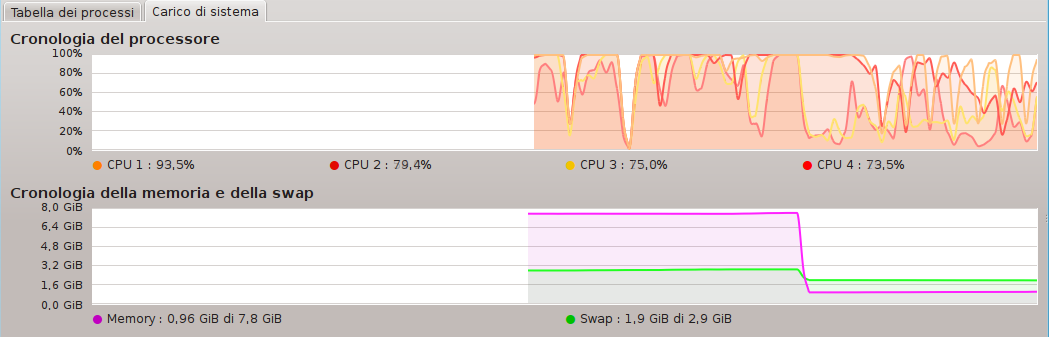
\includegraphics[width=1.0\textwidth]{assets/sib-memory-leak.png}
	\caption{Memory Leak del SIB che avveniva quando la connessione viene interrotta da un socket-timeout}
	\label{fig:sib-memory-leak}
\end{figure}

\noindent
La scoperta di questo problema ha portato quindi alla necessità di ottimizzare le performance, è stato quindi deciso di limitare il numero di risposte fornite dal servizio cittadino (Par. ~\ref{par:thread}) che causa un ingente traffico di dati da e verso il SIB. Altra ottimizzazione che decisa in seguito a queste scoperte è stata quella di trasformare le operazioni di INSERT di triple in query SPARQL, in quanto, grazie all'uso dei prefissi al posto degli URL interi, si riesce ad ottimizzare notevolmente il volume di dati scambiato, il che porta a notevoli vantaggi durante l'uso nell'applicazione mobile.










  
  \chapter{Applicazione Mobile}\label{chap:mobile-app}

In questo capitolo verrà presentato un esempio di applicazione mobile in grado di connettersi al \emph{City Service} e di eseguire le operazione di prenotazione e ritiro delle ricariche. Il suo scopo è permettere all'utente di interagire con la smart-city al fine di ridurre le problematiche derivanti dall'utilizzo di veicoli elettrici. La comunicazione avviene mediante i protocolli visti nella Sez. ~\ref{sec:protocol}.

Inizialmente era possibile eseguire solo operazioni di prenotazione e cancellazione di ricariche e funzionava unicamente in presenza del simulatore in quanto si prendeva il possesso di un veicolo simulato. Il funzionamento è stato poi ampliato con la possibilità di connettersi tramite Bluetooth a un veicolo reale, opportunità concessa dal \emph{Centro Ricerche Fiat} (\emph{CRF}), oppure di connettersi in assenza di veicoli per permettere all'utente di effettuare una ricarica comodamente seduto a casa.

A questo si è aggiunta la possibilità di analizzare il profilo altimetrico che separa il dispositivo mobile da un determinato EVSE con lo scopo di fare previsioni più accurate sui consumi necessari a raggiungerlo.

La piattaforma di sviluppo scelta è \emph{Android} vista la sua grandissima diffusione e versatilità.

\section{Architettura}

La piattaforma scelta per lo sviluppo è Android dalla versione \emph{4.0.3} in su. Questo perché vanta maggiori performance e un interfaccia utente più gradevole è facile da programmare. La libreria di base per interfacciarsi con il SIB è quella esposta nella sezione ~\ref{subsec:ioe-lib}.

La comunicazione con il servizio cittadino avviene tramite scambio di messaggi con il \emph{City SIB}, mentre le informazioni relative al veicolo, in particolar modo se quest'ultimo è simulato, arrivano dal \emph{Dash SIB}. È possibile collegare l'applicazione ad un veicolo reale che sia provvisto della tecnologia Blue\&{}Me di Fiat. I dati del profilo altimetrico sono ottenuti tramite una libreria, chiamata \emph{UniboGeoTools}, che ho sviluppato appositamente per l'occasione.

\subsection{Android}

Malgrado Android sia ampiamente conosciuto penso sia necessario spendere qualche parola al fine di introdurre i concetti che stanno alla base della programmazione di applicazioni su questo sistema operativo per poter capire approfonditamente il resto della trattazione.

Android è un sistema operativo basato Linux-based, Open Source, orientato all'utilizzo su dispositivi mobili anche se negli ultimi anni sta prendendo sempre più piede all'interno di smart-tv, dispositivi embedded, mini computer ecc..

La programmazione di applicazioni avviene attraverso una versione ad-hoc del linguaggio Java che, seppur venga eseguita su una virtual machine diversa dalla JVM (Dalvik), ne mantiene quasi tutte le caratteristiche e la libreria di base. Naturalmente oltre alla libreria standard vengono fornite le API che permettono l'interfacciamento con le funzionalità di Android.

\subsubsection{Activity}

Le Activity sono uno degli elementi centrali della programmazione di applicazioni Android (\cite{html:android}). In genere un Activity rappresenta una singola schermata della nostra applicazione. Le applicazioni possono definire una o più Activity per trattare diverse fasi del software, e generalmente ognuna di esse corrisponde ad un azione specifica che può essere eseguita dall'utente. 

Ci può essere una sola Activity attiva in un determinato istante, quelle che invece non sono attive possono essere terminate in qualunque momento dal sistema operativo al fine di recuperare memoria, questo comporta che il programmatore debba prevedere per ogni Activity il codice necessario a salvarne lo stato per permetterne il ripristino nel caso sia necessario. Questo comporta, come si può vedere in figura ~\ref{fig:android-activity}, che le Activity di Android abbiano un ciclo di vita abbastanza complesso. 

\subsubsection{Service}

Un Service è un processo che gira in background (un concetto molto simile al deamon in ambiente Unix) e può essere vviato e comandato da Activity o altri Service. La classe Service viene utilizzata per creare componenti software che possono svolgere attività in modo ``invisibile'', senza interfaccia utente.

Un Service può trovarsi in due stati(\cite{emanuele:android}):

\begin{itemize}
	\item \textbf{Started}: Un servizio si trova in questo stato quando viene invocato il metodo startService(), il servizio gira in background per un tempo indefinito o finché il componente che lo ha invocato non viene distrutto (Fig. ~\ref{fig:android-service} sinistra).
	\item \textbf{Bounded}: Un servizio si trova in questo stato quando si invoca il metodo bindService(). I servizi di questo tipo offrono un'interfaccia per la comunicazione client-server, in questo modo le componenti che invocano il servizio possono interagire con esso. In questo caso il servizio è attivo solo finché le componenti sono associate con esso (Fig. ~\ref{fig:android-service} destra).
\end{itemize}

\noindent
Un Servizio avviato ha una priorità più alta rispetto ad Activity in stato di inattività, in questo modo vi è minore probabilità per un Service di essere terminato dal gestore delle risorse di runtime. L’unica ragione per cui Android potrebbe fermare un Service prematuramente è per fornire risorse addizionali al componente software in primo piano (normalmente una Activity).

I servizi vengono avviati nel thread principale del processo, ciò significa che se eseguissero operazioni bloccanti o ad alto consumo di risorse potrebbero portare al blocco dell'intero processo e far generare ad Android un errore del tipo: ``Application Not Responding'', per evitare questo è bene far gestire il servizio in un thread separato.

\begin{figure}[H]
        \centering
        \begin{subfigure}[b]{0.49\textwidth}
			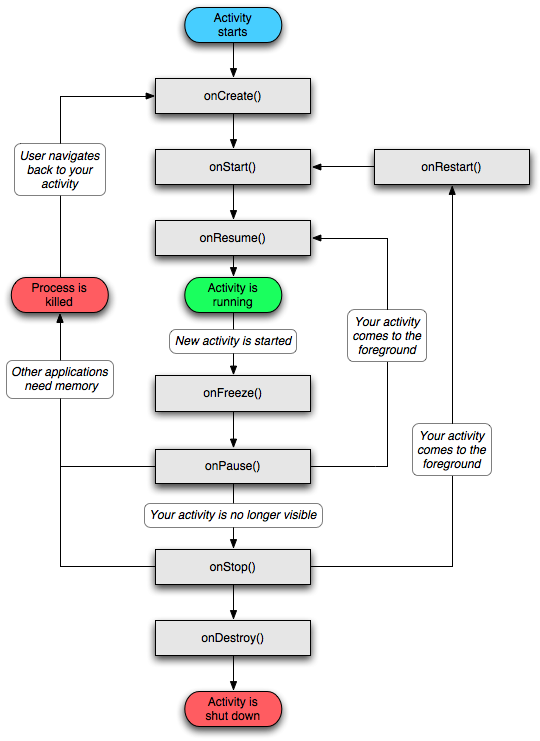
\includegraphics[width=\textwidth]{assets/android-activity.png}
			\caption{Ciclo di vita di un Activity Android}
			\label{fig:android-activity}
		\end{subfigure}
        \begin{subfigure}[b]{0.49\textwidth}
			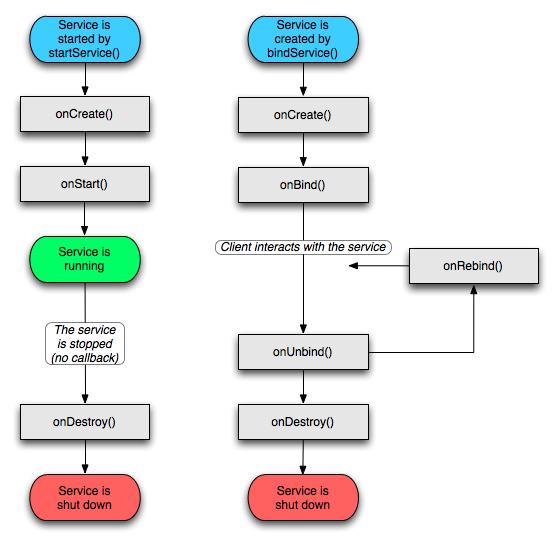
\includegraphics[width=\textwidth]{assets/android-service.png}
			\caption{Ciclo di vita di un Service Android}
			\label{fig:android-service}
		\end{subfigure}
        \caption{Ciclo di vita Activity e Service Android}
\end{figure}

\subsection{Blue\&{}Me}

Il Blue\&{}Me è il risultato di un accordo tra Fiat Auto e Microsoft con l'obiettivo di progettare sistemi telematici innovativi per l'automotive, il sistema è stato presentato nel 2006 (\cite{al2012android}). Basato sulla piattaforma Windows Embedded Automotive (unione del sistema operativo Windows CE con il middleware Microsoft Auto) è sviluppato da Magneti Marelli (azienda del gruppo FIAT) in collaborazione con Microsoft (\cite{wiki:blue-me}).

Blue\&{}Me è un sistema viva voce con tecnologia Bluetooth, riconoscimento vocale, lettore multimediale con presa USB e comandi al volante. Fiat Auto e Microsoft, con il supporto di Magneti Marelli, offrono una piattaforma adattabile alla maggior parte dei telefoni cellulari e lettori musicali. Il sistema si interfaccia al cellulare mediante la tecnologia Bluetooth e permette al guidatore di rispondere al telefono lasciando il telefono in tasca. 

La funzionalità del Blue\&{}Me più importante ai nostri scopi è la possibilità di monitorare i parametri del veicolo. Nel nostro caso abbiamo lavorato con un prototipo di Fiat Daily elettrico opportunamente modificato per trasmettere i dati della batteria tramite tecnologia Bluetooth. La connessione è stata possibile grazie a delle librerie fornite dal CRF con tanto di applicazione di esempio.

L'interazione con il Blue\&{}Me è di tipo push ovvero ogniqualvolta che la centralina della macchina si accorge che un dato è variato (secondo una determinata soglia) allora lo ``scrive'' sull'interfaccia Bluetooth. Il che implica che se dall'altra parte ci deve essere un applicazione che dedica un processo alla sola lettura delle informazioni che arrivano dal Blue\&{}Me. Fiat, nella libreria fornita, mette a disposizione un Service Andorid adatto allo scopo.

\subsection{Profilo Altimetrico e Contributo Energetico}

Grazie allo sviluppo di un apposita libreria, UniboGeoTools (App. ~\ref{app:unibo-geo-tools}) l'applicazione è in grado di prelevare i dati relativi al profilo altimetrico che separa l'utente da una determinata destinazione e quindi fare uno studio sul contributo energetico necessario a vincere il dislivello. Le informazioni riguardo al consumo energetico sono approssimative ma danno comunque un indicazione valida all'utente il quale se vede che l'energia necessaria a vincere il dislivello è maggiore di quella contenuta nella batteria allora saprà per certo che in quel determinato punto non ci potrà arrivare.

La libreria UniboGeoTools possiede anche funzioni utili a trovare il percorso, in strada, tra due punti. Queste si sono rivelate particolarmente utili al fine di mostrare i percorsi sulla mappa e la distanza precisa che separa l'utente, ad esempio, da una colonnina di ricarica.


\section{Modalità di esecuzione}

L'applicazione al fine di adattarsi ai diversi scenari possibili offre molteplici modalità di esecuzione, questo per adattarsi a tutti gli scenari possibili. La scelta della modalità di esecuzione avviene nella schermata iniziale come si può vedere in figura ~\ref{fig:main-activity}

\begin{figure}
	\centering
	\begin{subfigure}{0.45\textwidth}
		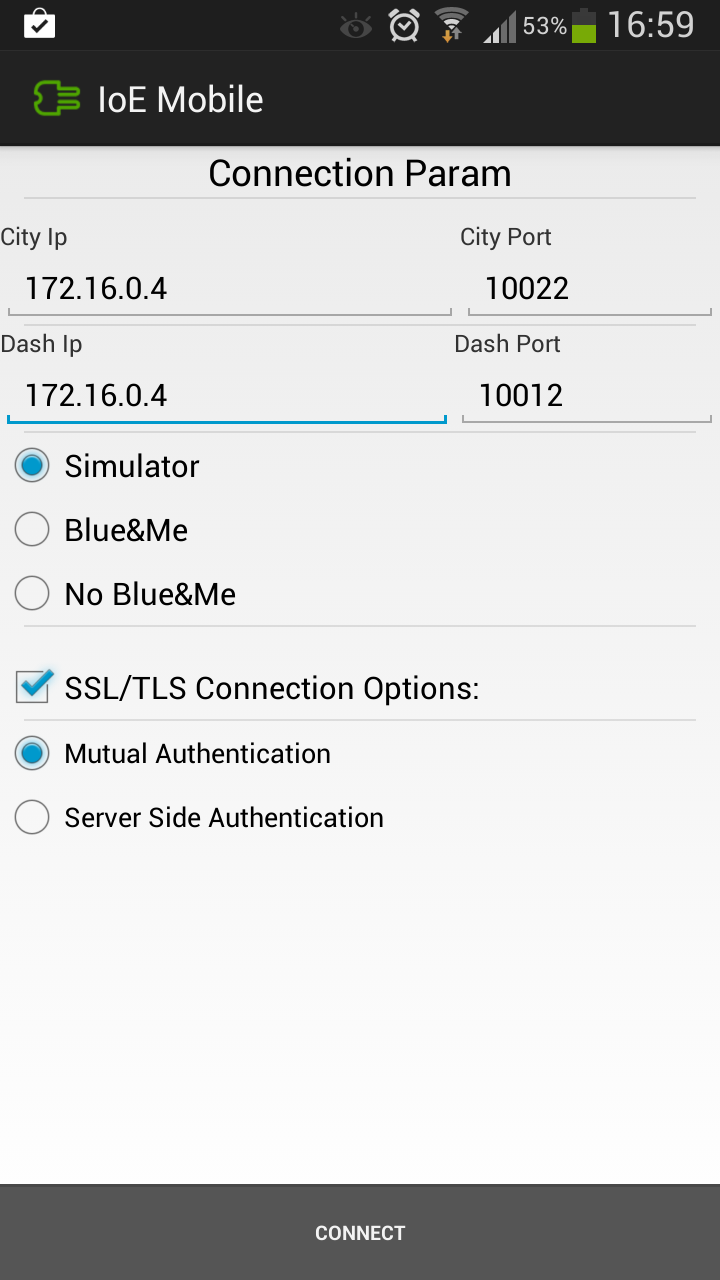
\includegraphics[width=\textwidth]{assets/mobile-app-main.png}
		\caption{Schermata Principale}
		\label{fig:main-activity}
	\end{subfigure}
	\begin{subfigure}{0.45\textwidth}
		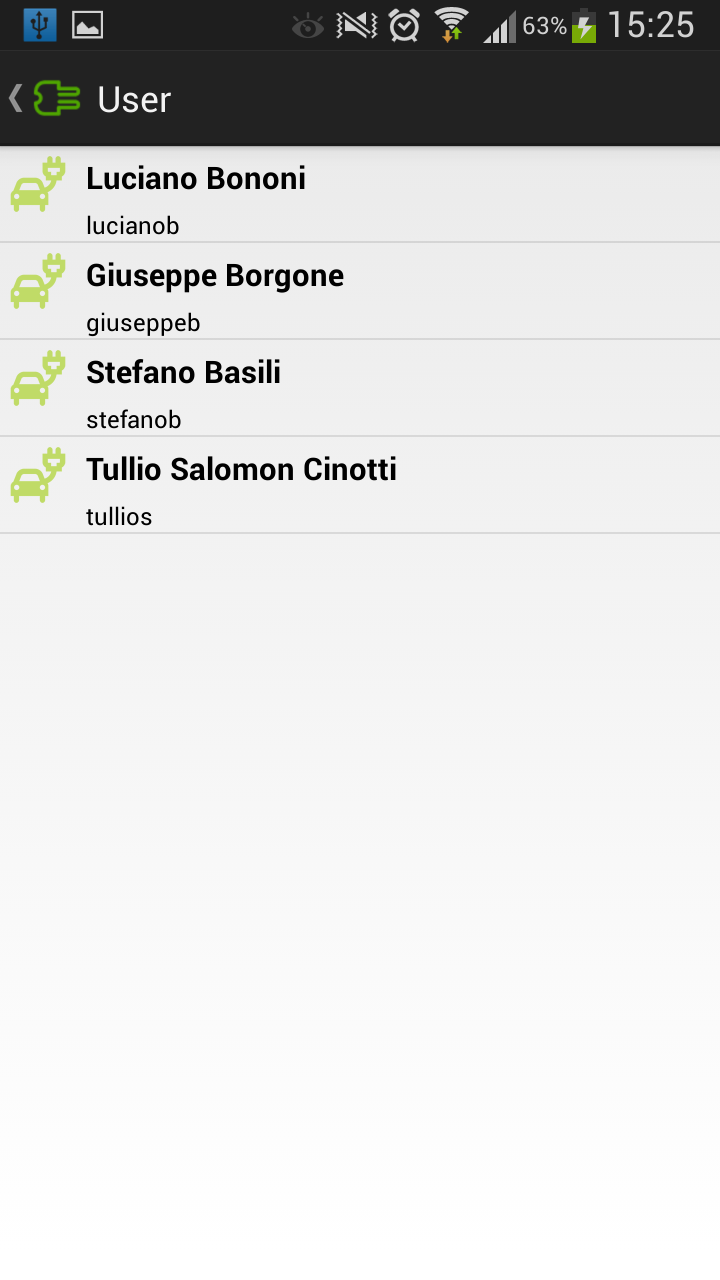
\includegraphics[width=\textwidth]{assets/mobile-app-select-user.png}
		\caption{Selezione Utente}
		\label{fig:select-user}
    \end{subfigure}
    	\begin{subfigure}{0.45\textwidth}
		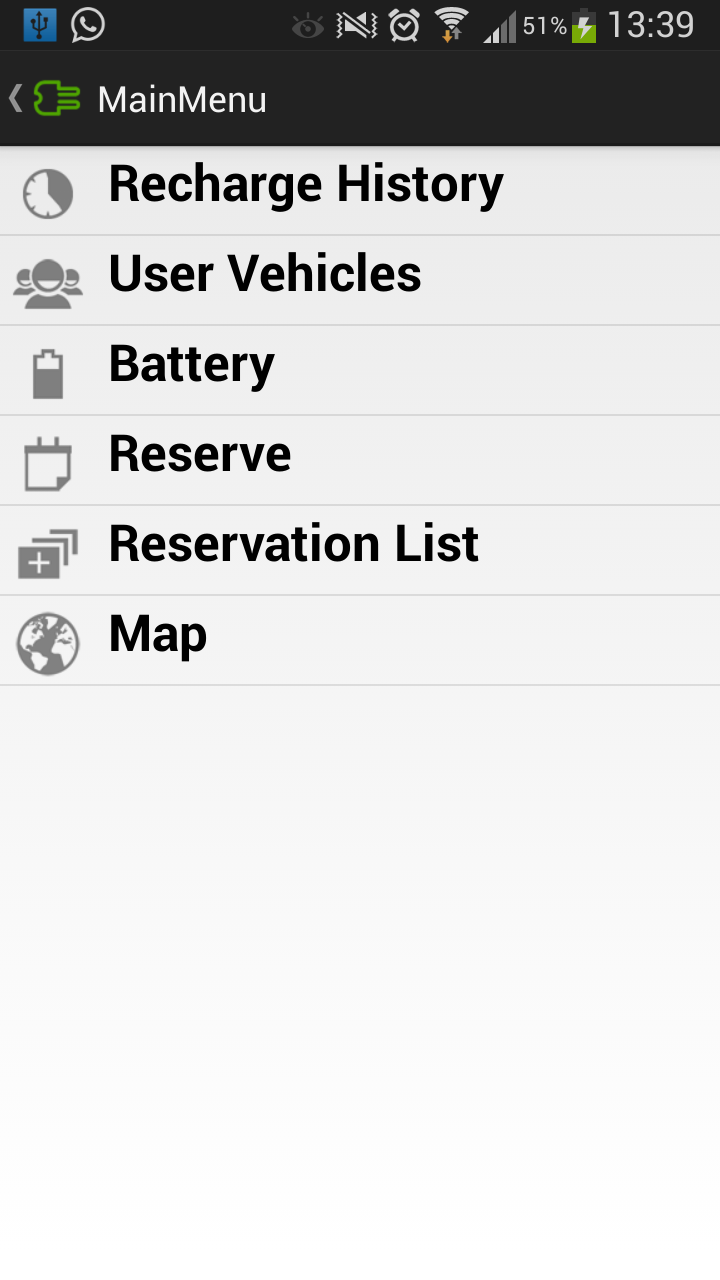
\includegraphics[width=\textwidth]{assets/mobile-app-main-menu.png}
		\caption{Menu Principale}
		\label{fig:main-menu}
	\end{subfigure}
	\begin{subfigure}{0.45\textwidth}
		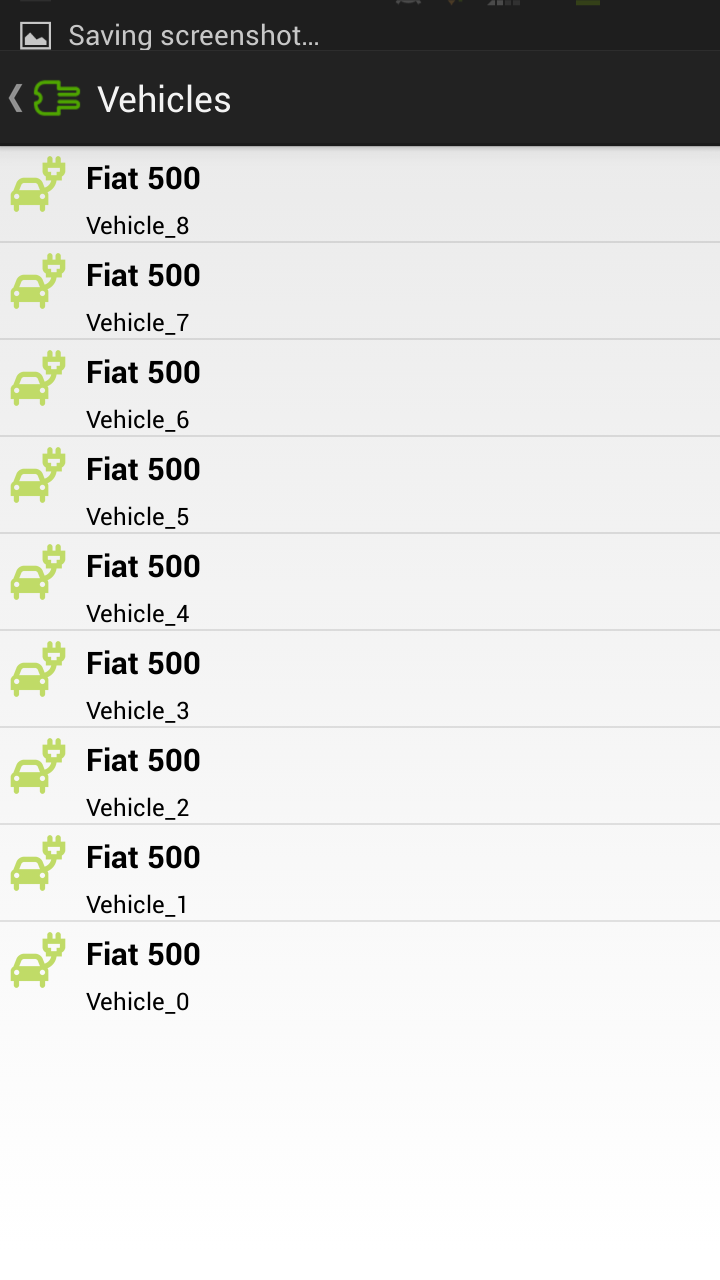
\includegraphics[width=\textwidth]{assets/mobile-app-select-veh.png}
		\caption{Selezione Veicolo}
		\label{fig:select-veh}
    \end{subfigure}
\end{figure}

\subsection{Simulazione}

Questa modalità permette di prendere il controllo di un veicolo contenuto nel simulatore, il quale deve essere avviato con un apposito parametro che causa la scrittura dei dati relativi ai veicoli sul \emph{Dash SIB}. Questo implica che una volta premuto sul pulsante \emph{Connect} (Fig. ~\ref{fig:main-activity}), bisogna scegliere "Luciano Bononi" in quanto è l'utente di default usato dalle macchine del simulatore (Fig. ~\ref{fig:select-user}). Da qui in poi l'applicazione non ha molte differenze rispetto alla modalità di esecuzione con Blue\&{}Me se non che le azioni intraprese avranno ripercussioni sul simulatore e non sul mondo reale.

\subsection{Con Blue\&{}Me}

Questa modalità viene usata in un contesto reale e necessita la presenza di un veicolo che possegga la tecnologia Blue\&{}Me di Fiat. Le informazioni relative alla batteria vengono prelevate tramite Bluetooth scritte nel \emph{Dash SIB} per i motivi di interoperabilità spiegati nella Sez. ~\ref{subsec:dash-sib} ovvero dare la possibilità a chiunque di interfacciarsi con l'applicazione mobile a patto di scrivere un adattatore che scriva i dati sulla \emph{Dash SIB}. Le informazioni relative al GPS, siccome non fornite dal veicolo, vengono prelevati dal GPS (o altre fonti) fornito dallo smartphone.

\subsection{Senza Blue\&{}Me}\label{subsec:noblueme}

Questa modalità d'uso è rivolta principalmente a chi vuole svolgere le attività di interazione con il \emph{City Service} senza essere a bordo del proprio veicolo. Questo comporta l'assenza della \textsc{Dash SIB}, infatti quando viene scelta viene disabilitato l'inserimento dei parametri di quest'ultima. Diviene quindi impossibile monitorare i parametri del veicolo e di conseguenza parte del menu principale viene disabilitata. Anche se la \emph{Dash SIB} fosse situata sul cellulare anziché sul veicolo a poco servirebbe in quanto il veicolo sarebbe comunque fuori portata o comunque spento. Si possono comunque svolgere le operazioni di prenotazione e ritiro delle ricariche e tenere monitorato lo stato di quelle già effettuate nonché guardare la mappa con le colonnine.


\section{Funzionalità}

In questa sezione eseguirò un analisi dettagliata delle funzionalità dell'applicazione. La descrizione cercherà di essere il più possibile funzionalità-centrica e non activity-centrica anche se spesso le due cose coincidono. 

%Questo significa che a partire dalle funzionalità cercherò di introdurre le Activity coinvolte nello svolgimento.
%Le Activity si trovano nel package \code{it.unibo.ioe.activities}, nel package \code{it.unibo.ioe.activities.maps} invece si trovano le Activity destinate alla gestione delle mappe e infine nel package \code{it.unibo.ioe.services} troviamo i servizi. 

\subsection{Il menu principale}

La prima schermata dell'applicazione è quella che permette di scegliere i parametri di connessione ai SIB (Fig. ~\ref{fig:main-activity})  e la modalità di esecuzione. Una volta premuto il tasto \emph{connect} ci troveremo a scegliere l'utente (Fig. ~\ref{fig:select-user}) a questo punto ci troveremo davanti il menu principale (Fig. ~\ref{fig:main-menu}).

Il menu apparirà con solo due opzioni: \emph{Recharge History} e \emph{Select Vehicle}. Questo perché tutte le altre opzioni sono subordinate al veicolo che si sta utilizzando e quindi non vengono mostrate finché non se ne sceglie uno attraverso l'apposito menu (Fig. ~\ref{fig:select-veh}). 

\subsection{Storia delle ricariche effettuate}

In questa schermata (Fig. ~\ref{fig:recharge-history}) possiamo tener monitorata la storia delle ricariche effettuate. Questa parte è stata introdotta anche per dimostrare l'interoperabilità del nostro sistema con uno SIB-based sviluppato dalla spagnola AICIA.

\subsection{Monitoraggio Parametri Batteria}

Dal menu principale si può accedere al monitoraggio dei parametri della batteria attraverso l'opzione \emph{Battery}. Il monitoraggio consente di vedere sia i parametri variabili (Fig. ~\ref{fig:battery-var}) che quelli nominali (Fig. ~\ref{fig:battery-nom}). I dati relativi all'intensità di corrente e al voltaggio sono visibili solo se si è connessi a un veicolo reale tramite Blue\&{}Me in quanto il nostro modello di simulazione non li implementa. Mentre i dati nominali sono disponibili in modalità di simulazione ma non in quella reale in quanto queste informazioni non vengono fornite dalla centralina del veicolo.

\begin{figure}
	\centering
	\begin{subfigure}{0.45\textwidth}
		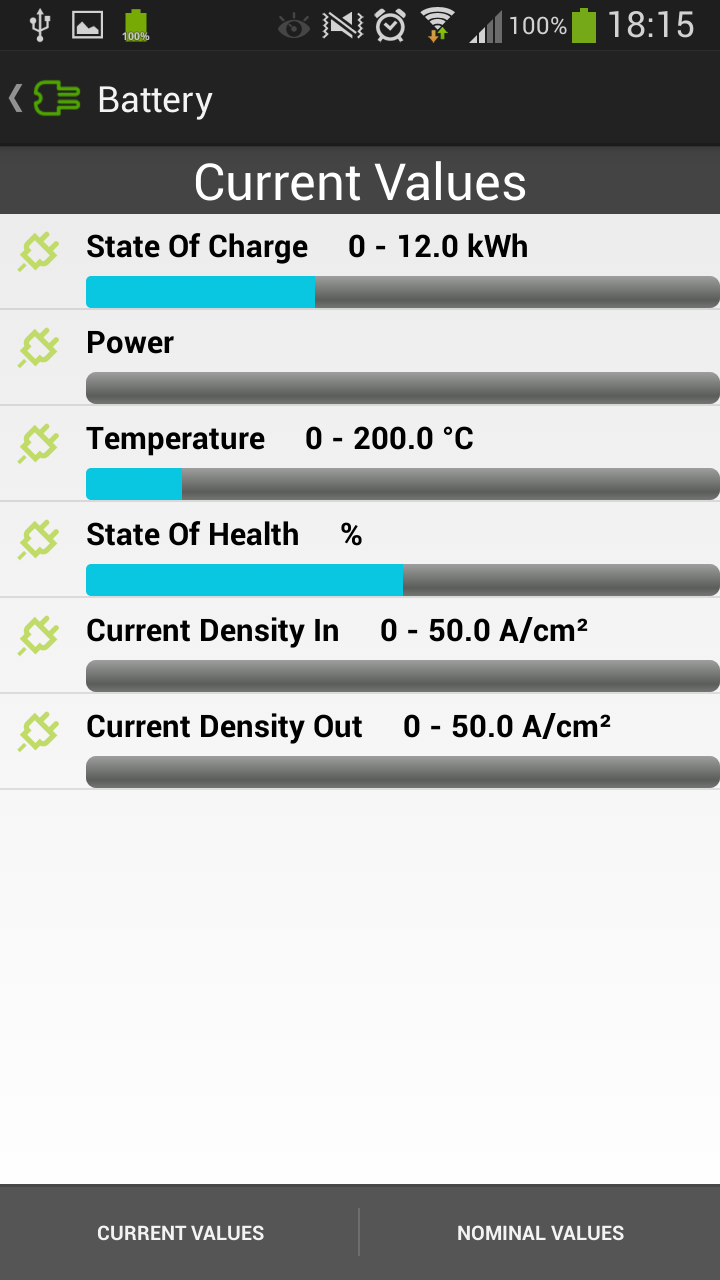
\includegraphics[width=\textwidth]{assets/mobile-app-battery-var.png}
		\caption{Dati variabili della batteria}
		\label{fig:battery-var}
	\end{subfigure}
	\begin{subfigure}{0.45\textwidth}
		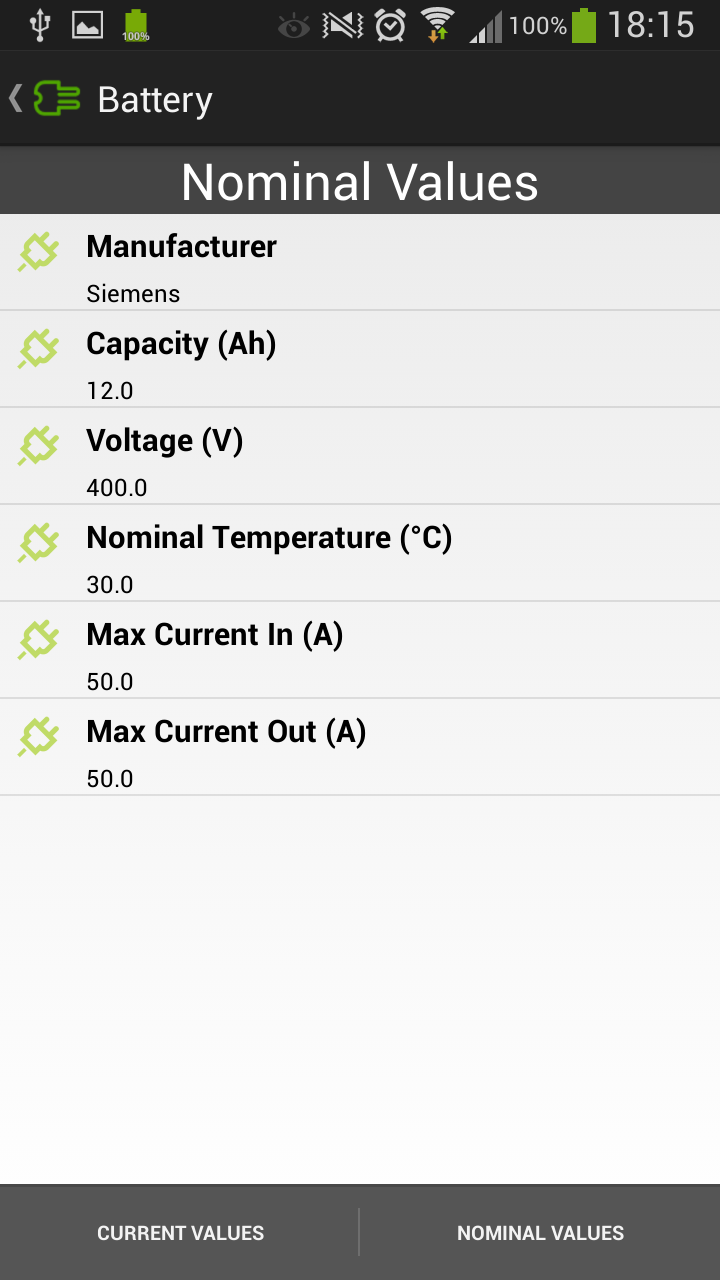
\includegraphics[width=\textwidth]{assets/mobile-app-battery-nom.png}
		\caption{Dati fissi della batteria}
		\label{fig:battery-nom}
    \end{subfigure}
    \begin{subfigure}{0.45\textwidth}
		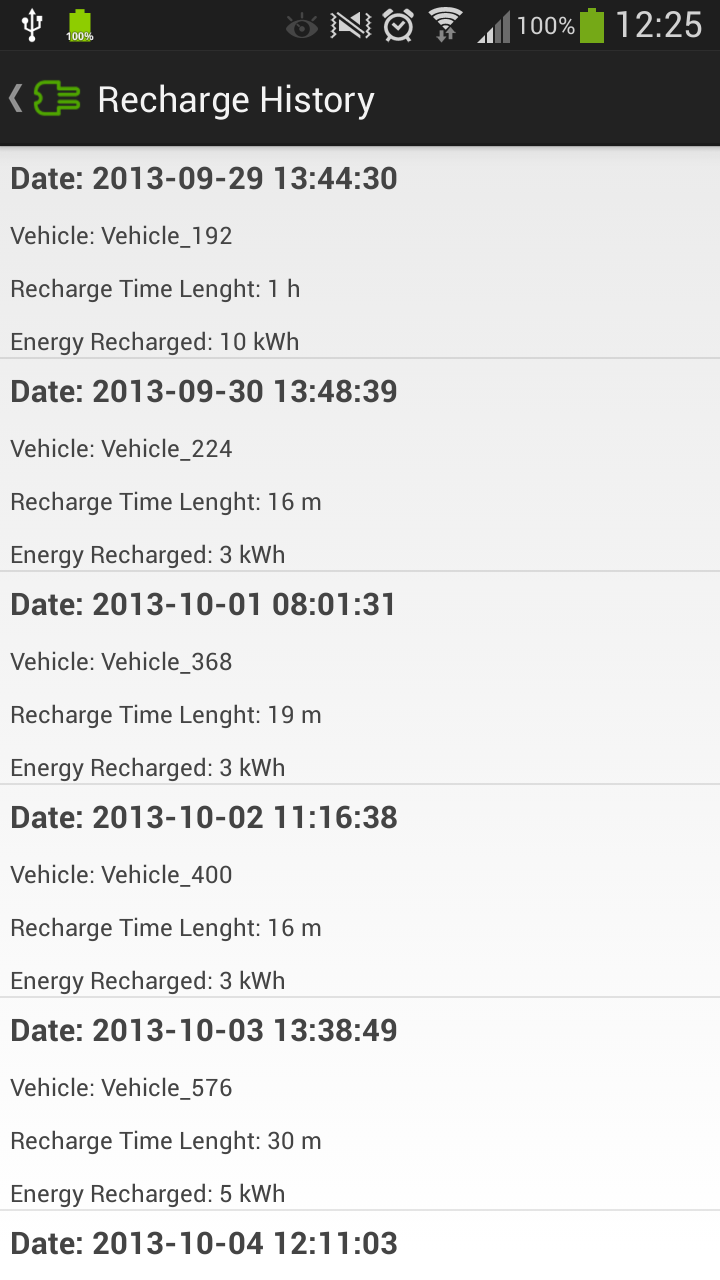
\includegraphics[width=\textwidth]{assets/mobile-app-recharge-history.png}
		\caption{Storia Ricariche}
		\label{fig:recharge-history}
	\end{subfigure}
	\begin{subfigure}{0.45\textwidth}
		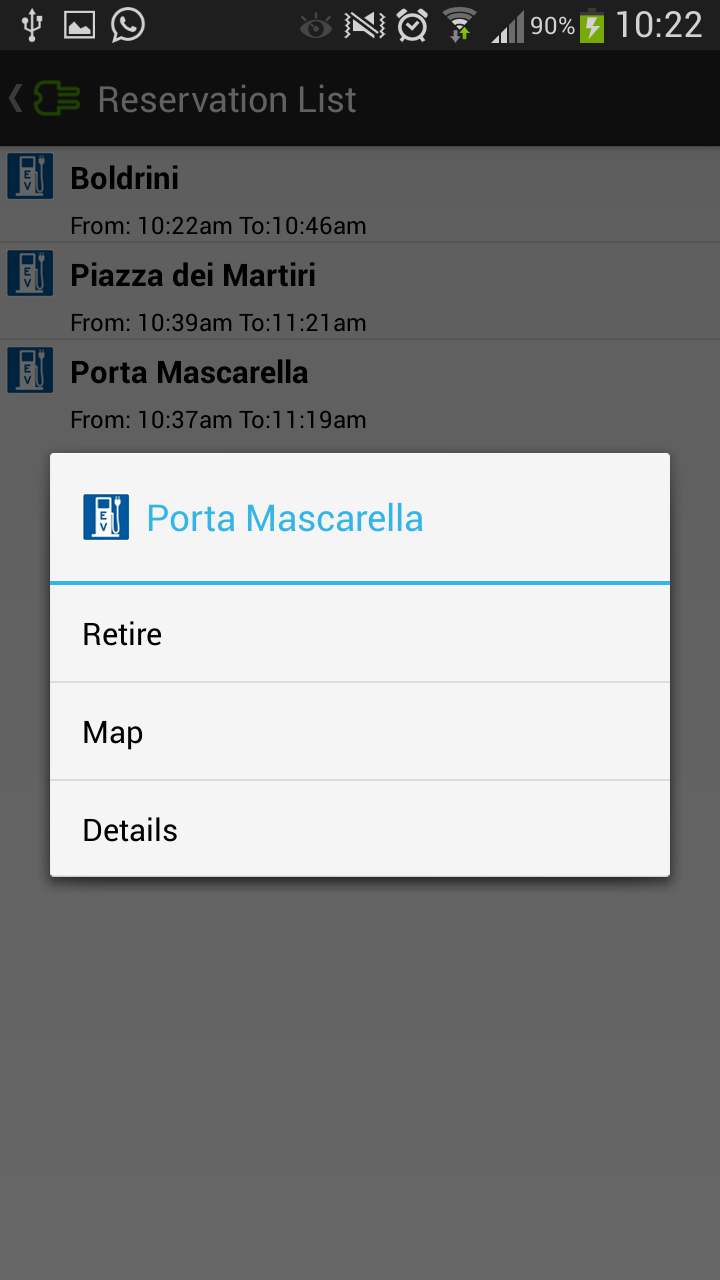
\includegraphics[width=\textwidth]{assets/mobile-app-reservation.png}
		\caption{Selezione Veicolo}
		\label{fig:reservation}
    \end{subfigure}
\end{figure}

\subsection{Effettuare una richiesta di prenotazione}

Per accedere a questa funzionalità bisogna scegliere dal menu principale l'opzione \emph{Reserve}. Ci troveremo davanti alla schermata che ci permette di impostare i parametri necessari a creare una richiesta di prenotazione. Come si può vedere in figura ~\ref{fig:charge-request} il servizio mette a disposizioni svariate opzioni per personalizzare il processo di prenotazione. Essenzialmente in questa schermata viene data una veste grafica al protocollo di richiesta descritto nella sezione ~\ref{sec:protocol}.

\subsubsection{Creazione della richiesta}

La scelta dell'area dentro la quale cercare le colonnine assume di default la posizione del veicolo come punto centrale, nel caso essa non sia disponibile (modalità \emph{Senza Blue\&{}Me}, Sez. ~\ref{subsec:noblueme}) allora l'utente è costretto a sceglierne dalla mappa. Per accedere alla funzione di scelta del punto si clicca sul pulsante \emph{Map} il quale mostra apre la mappa centrata sulla città in cui ci troviamo e tramite un tocco sullo schermo permette di scegliere il punto di interesse (Fig ~\ref{fig:map-chooser}).

Una volta scelto centrata la nostra area di interesse si procede scegliendo il raggio di ricerca. Di default è impostato a 6 e al massimo si può impostare a 15, di più non avrebbe senso visto che in linea di massima si sposta il punto di interesse.

La barra che permette di scegliere la quantità di energia ha come dimensione massima la capacità della batteria. Nell'immagine in Fig. ~\ref{fig:charge-request} abbiamo una batteria con capacità 40kWh e una quantità di energia residua di 12kWh, questo si capisce dal colore rosso del numero a destra della barra che indica che stiamo tentando di acquistare 0kWh. Spostando la barra verso destra andremo a indicare fino a che punto volgiamo ricaricare la batteria, il numero a destra a questo punto diventa nero. Non si può procedere finché non si acquista almeno 1kWh. 
Nel caso in cui la capacità e la quantità di carica non siano disponibili allora viene data la possibilità di scegliere qualunque quantità di energia, l'utente viene però messo in guardia del fatto che potrebbe acquistare più energia di quella che può contenere la batteria del veicolo.

L'ultimo parametro da impostare è l'intervallo di tempo in cui siamo disposti a ricaricarci. Di default viene proposto un lasso temporale di 3 ore. È possibile variarlo premendo sui pulsanti nel quale è scritta la data i quali mostreranno un calendario e un selettore di orario. Ovviamente sono stati messi dei controlli che impediscono di mettere orari incoerenti come ora di inizio successiva a quella di fine.

A questo punto possiamo inviare la richiesta premendo l'apposito pulsante in alto a destra.

\subsubsection{Scelta della risposta}

In seguito all'invio della richiesta viene mostrato all'utente un messaggio che invita ad attendere la risposta. Nel caso la richiesta sia fallita allora l'utente viene allertato e rimandato nella schermata di prenotazione con l'invito di cambiare i parametri.

In caso di successo viene mostrata una schermata con tutte le opzioni di ricarica restituite dal servizio cittadino. Come si può vedere in Fig. ~\ref{fig:charge-options} vengono fornite diverse informazioni per ognuna di esse:

\begin{itemize}
	\item Nome del GCP presso cui avverrà la ricarica.
	\item Distanza reale dal GCP, calcolata grazie alla libreria UniboGeoTools.
	\item Orario e prezzo della ricarica.
	\item Energia stimata per raggiungere la colonnina.
	\item Dislivello in salita e in discesa.
\end{itemize}

Le informazioni sul profilo altimetrico ed il contributo energetico vengono mostrate in una schermata a parte accessibile tramite un apposito menu visualizzabile tenendo premuta a lungo un opzione di ricarica (Fig. ~\ref{fig:charge-options-menu}), questo aspetto verrà approfondito in una sezione a parte (~\ref{subsec:altimetry}).

Viene data inoltre la possibilità di eseguire operazioni di ordinamento delle varie ricariche in base ai parametri sopra elencati ovvero: distanza, prezzo, orario, contributo energetico ecc.. Infine volendo si possono guardare le opzioni di ricarica sulla mappa. Premendo su una di esse viene disegnato il percorso necessario ad arrivarci con la particolarità che i tratti in salita sono colorati di rosso, quelli in discesa di verde e infine quelli in pianura di grigio. Le caratteristiche della mappa sono comunque approfondite nella Sez. ~\ref{subsec:map}.

Scegliendo l'opzione di ricarica viene eseguita la parte restante del protocollo, e nel caso in cui sia ancora valida allora verremo mandati alla schermata che presenta le prenotazioni attive per l'utente (Fig. \ref{fig:reservation}).

\subsection{Visualizzazione e Ritiro delle Prenotazioni}

In questa schermata vengono visualizzate le prenotazioni pendenti per l'utente (Fig. \ref{fig:reservation}). Vi si può accedere tramite il menu principale \emph{Reservation List} oppure ci si viene portati direttamente se viene confermata dal sistema l'opzione di ricarica scelta durante il processo di prenotazione. 

Selezionando una delle prenotazioni apparirà un menu che permette di mostrarla sulla mappa oppure di ritirarla.

\begin{figure}
	\centering
	\begin{subfigure}{0.45\textwidth}
		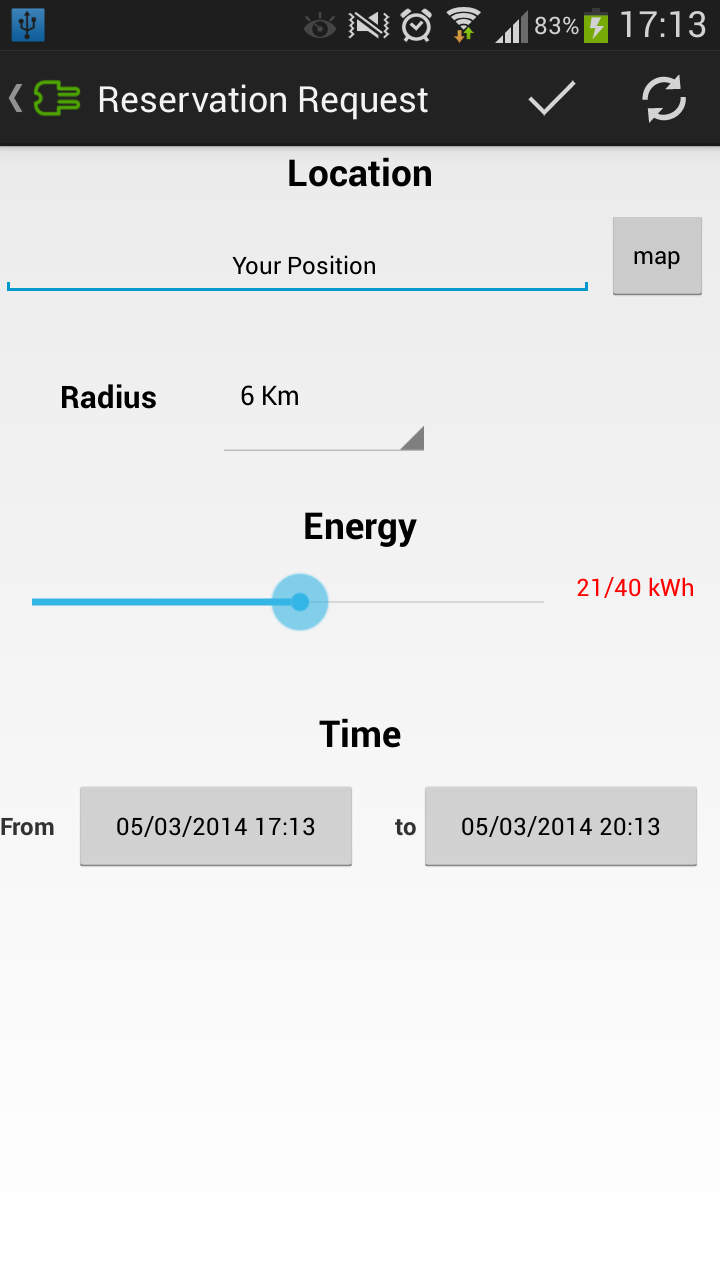
\includegraphics[width=\textwidth]{assets/mobile-app-charge-request.png}
		\caption{Inserimento Prenotazione}
		\label{fig:charge-request}
	\end{subfigure}
	\begin{subfigure}{0.45\textwidth}
		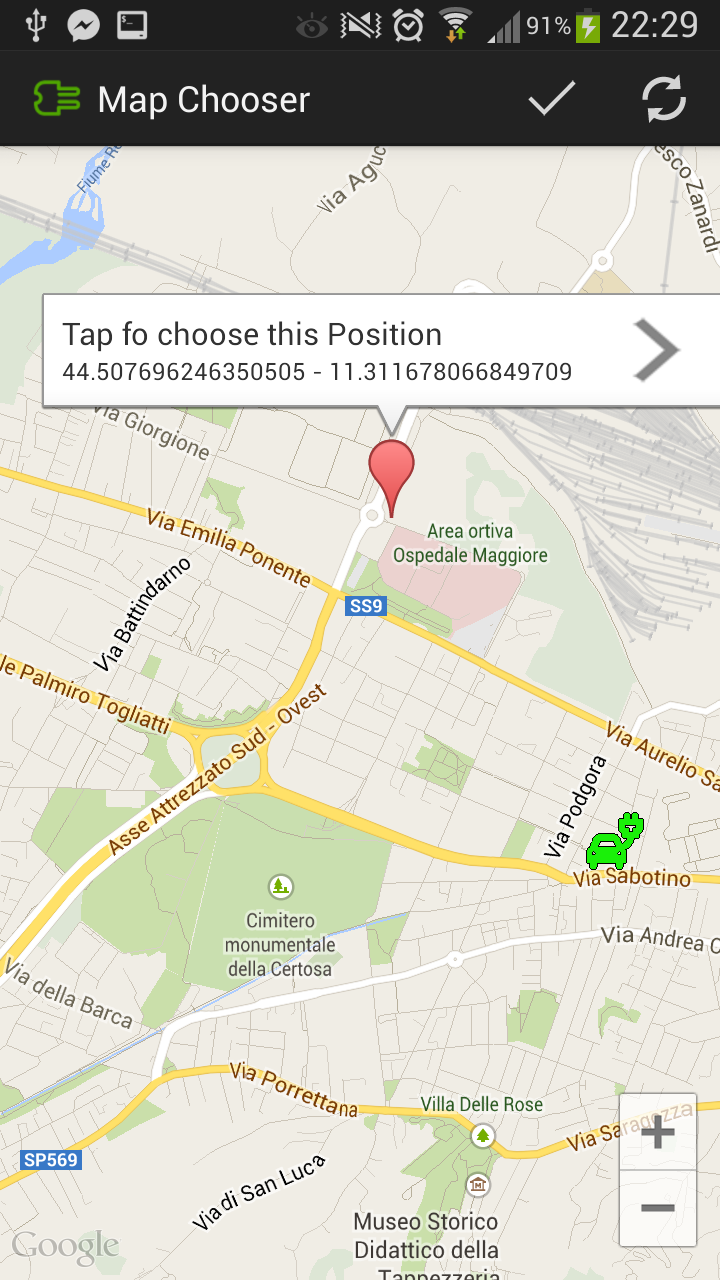
\includegraphics[width=\textwidth]{assets/mobile-app-map-chooser.png}
		\caption{Scelta di un punto nella mappa}
		\label{fig:map-chooser}
	\end{subfigure}
	\begin{subfigure}{0.45\textwidth}
		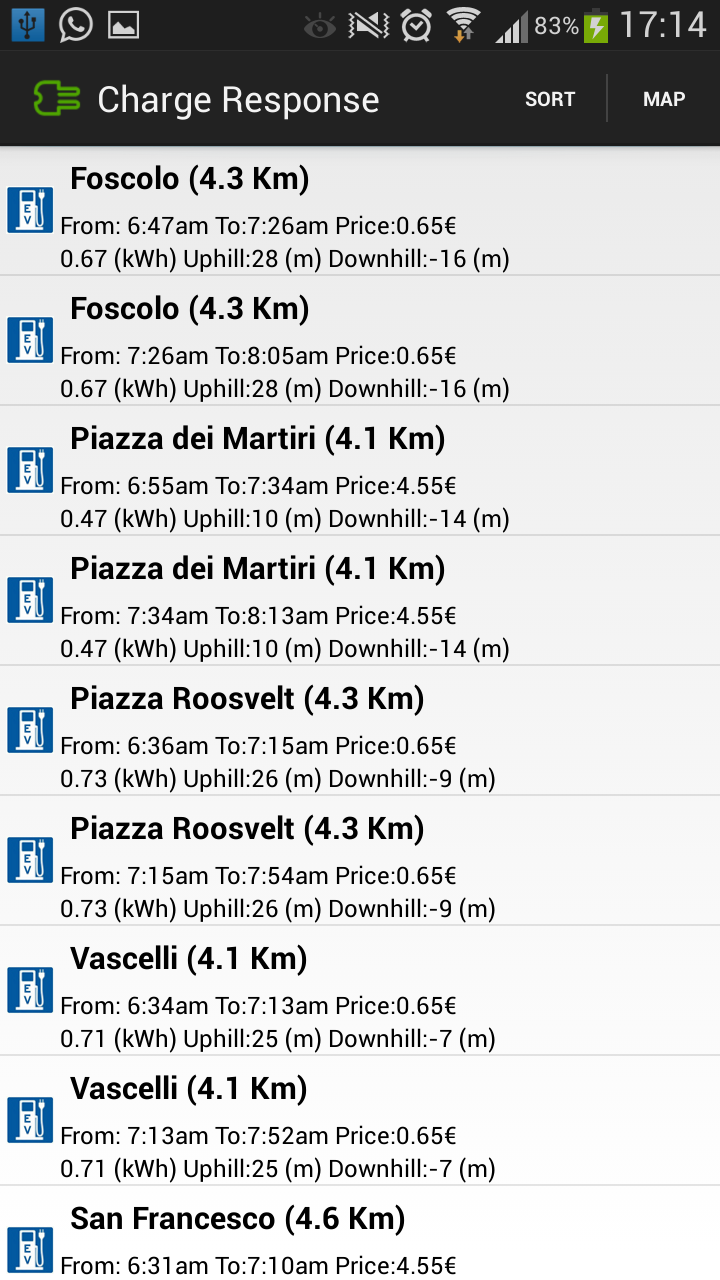
\includegraphics[width=\textwidth]{assets/mobile-app-charge-options.png}
		\caption{Visualizzazione opzioni di ricarica}
		\label{fig:charge-options}
    \end{subfigure}
	\begin{subfigure}{0.45\textwidth}
		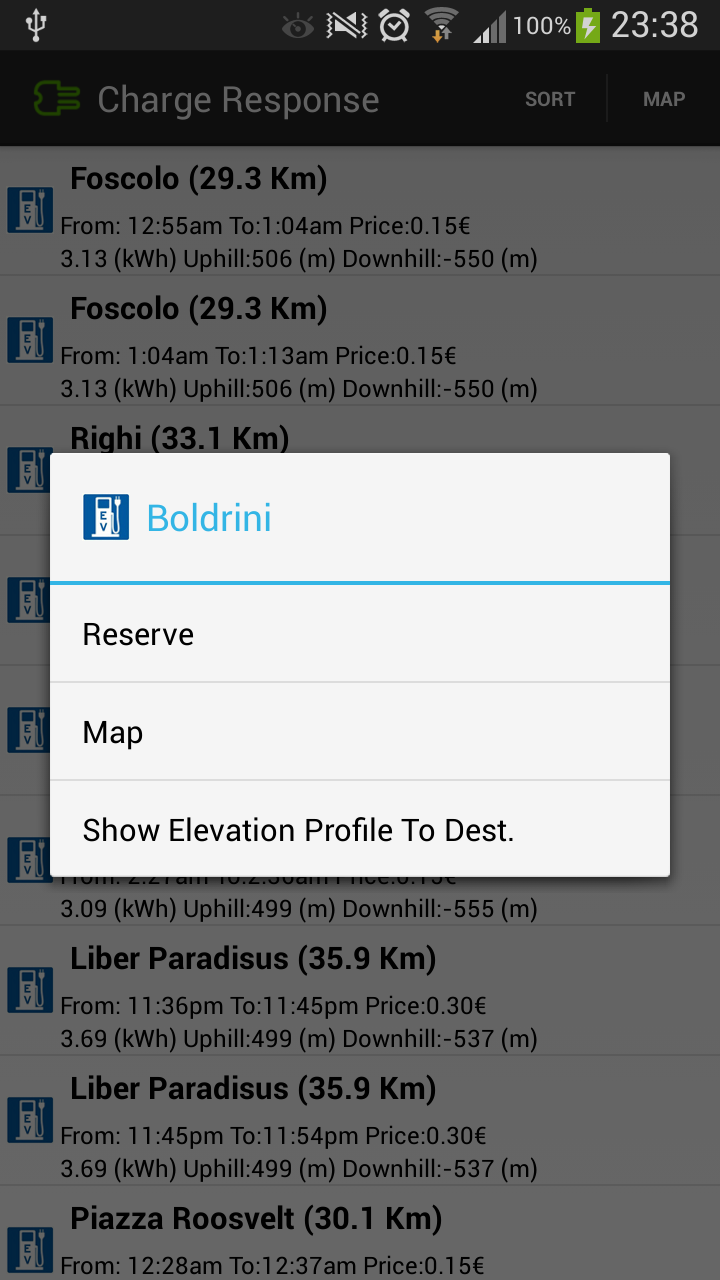
\includegraphics[width=\textwidth]{assets/mobile-app-charge-options-menu.png}
		\caption{Menu opzioni di ricarica}
		\label{fig:charge-options-menu}
    \end{subfigure}
\end{figure}

\subsection{Profilo Altimetrico e Contributo Energetico}\label{subsec:altimetry}

Il profilo altimetrico è una delle feature più innovative introdotte nell'applicazione. Può rivelarsi di fondamentale importanza nelle scelte dell'utente il quale, grazie ad essa, potrà scegliere il percorso migliore al fine di raggiungere la sua destinazione. Come vedremo nella sezione relativa al modello della batteria (\ref{sec:battery}), i veicoli elettrici hanno la possibilità di recuperare energia grazie alla frenata rigenerativa e al recupero in discesa. Questo significa che scegliere una strada con molti tratti in discesa può portare un recupero di energia non indifferente. 

La libreria UniboGeoTools, usata a questo scopo, permette inoltre di fare delle stime sull'energia necessaria a percorre un determinato tratto di strada. Queste informazioni sono mostrate nella schermata \emph{Elevation Profile}:

\begin{itemize}
	\item \textbf{Path Altimetry Summary}: Informazioni riassuntive sul viaggio che stiamo per intraprendere. Come si può vedere in Fig. ~\ref{fig:altimetry-1}, al di la delle informazioni di destinazione, distanza e peso, viene fornita una stima sull'energia totale che impiegherà il veicolo a raggiungere la destinazione, insieme alle informazioni su quanta discesa, salita e pianura compongo il percorso.
	\item \textbf{Cumulative Altimetry Offset}: In questo riquadro vengono fornite informazioni sul dislivello che caratterizza il percorso (Fig ~\ref{fig:altimetry-1}).
	\item \textbf{Average Slope}: Fornisce informazioni sulla pendenza media che caratterizza il percorso. Importante in quanto, come detto prima, una pendenza molto elevata può portare ad elevati consumi oppure a un ricavo di energia (Fig ~\ref{fig:altimetry-1}).
	\item \textbf{Max Slope}: Fornisce informazioni di massima sulla pendenza del percorso, ovvero la pendenza massimo che troveremo in salita e in discesa (Fig ~\ref{fig:altimetry-2}).
	\item \textbf{Elevation Dependent Energy Ref}: Informazioni sul contributo energetico impiegato per vincere il dislivello. A tal scopo viene utilizzata l'energia potenziale gravitazionale (Fig ~\ref{fig:altimetry-2}).
	\item \textbf{Energy Profile for Path Lenght}: Energia impiegata per percorrere il tragitto. Mentre nel caso precedente veniva preso in considerazione unicamente il dislivello qui viene considerata anche la distanza che ci separa dalla destinazione (Fig ~\ref{fig:altimetry-2}).
	\item \textbf{Altitude Graph}: Grafico che mostra il profilo altimetrico che ci separa dalla destinazione. I tratti in discesa sono in verde mentre quelli in salita in rosso (Fig ~\ref{fig:altimetry-3}).
\end{itemize} 
\noindent
Ulteriori informazioni sul profilo altimetrico vengono date sulla mappa aspetto approfondito nella Sez. ~\ref{subsec:map}.

\begin{figure}
	\centering
	\begin{subfigure}{0.45\textwidth}
		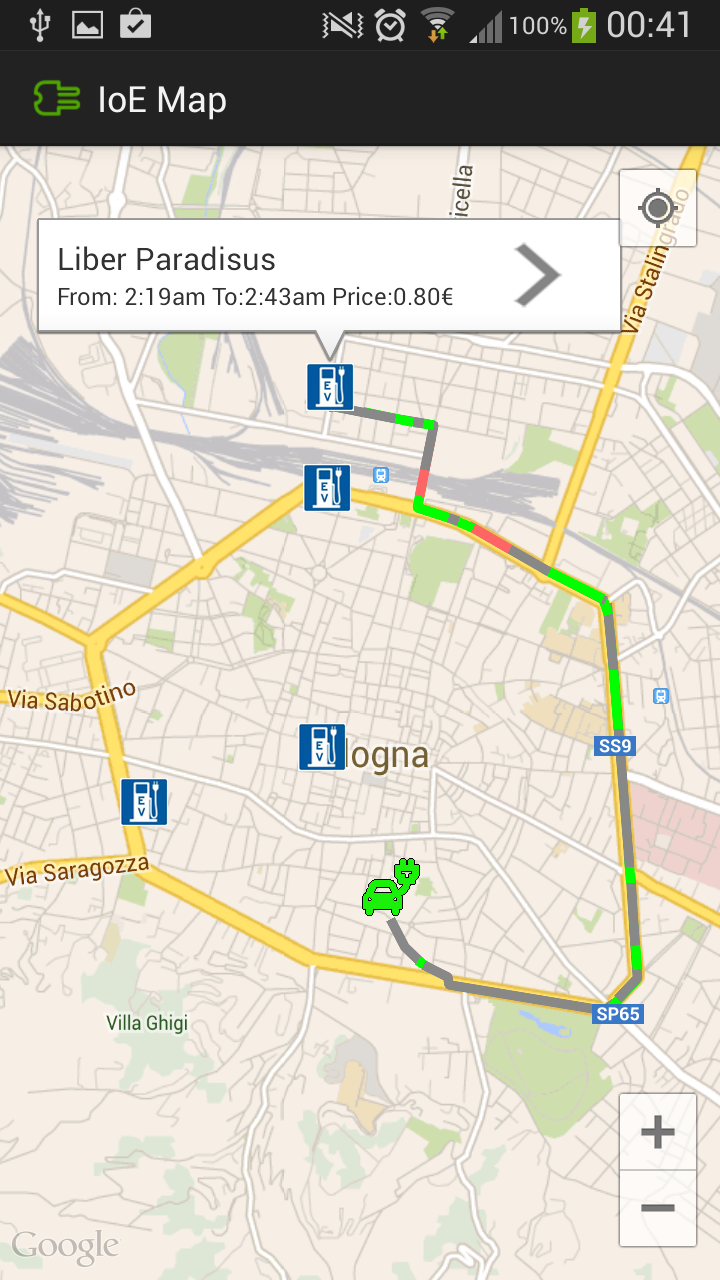
\includegraphics[width=\textwidth]{assets/mobile-app-map.png}
		\caption{Mappa con Profilo Altimetrico}
		\label{fig:map-altimetry}
	\end{subfigure}
	\begin{subfigure}{0.45\textwidth}
		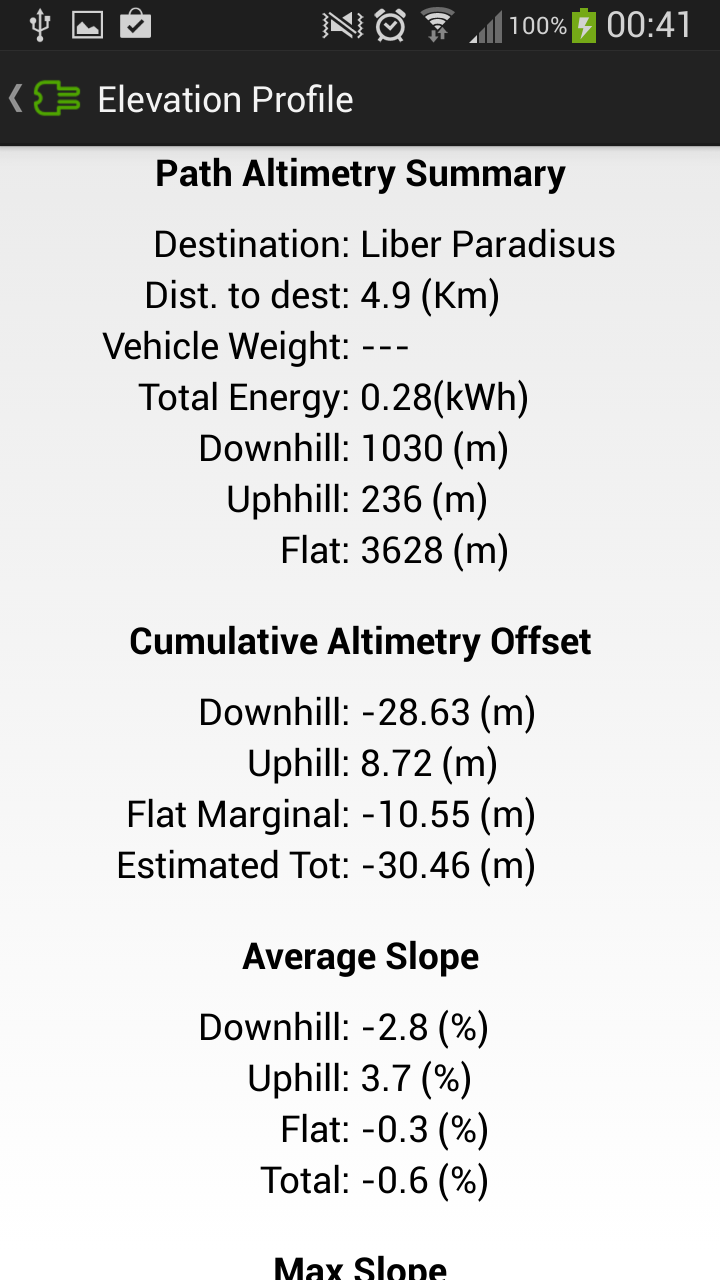
\includegraphics[width=\textwidth]{assets/mobile-app-altimetry-1.png}
		\caption{Scelta di un punto nella mappa}
		\label{fig:altimetry-1}
	\end{subfigure}
	\begin{subfigure}{0.45\textwidth}
		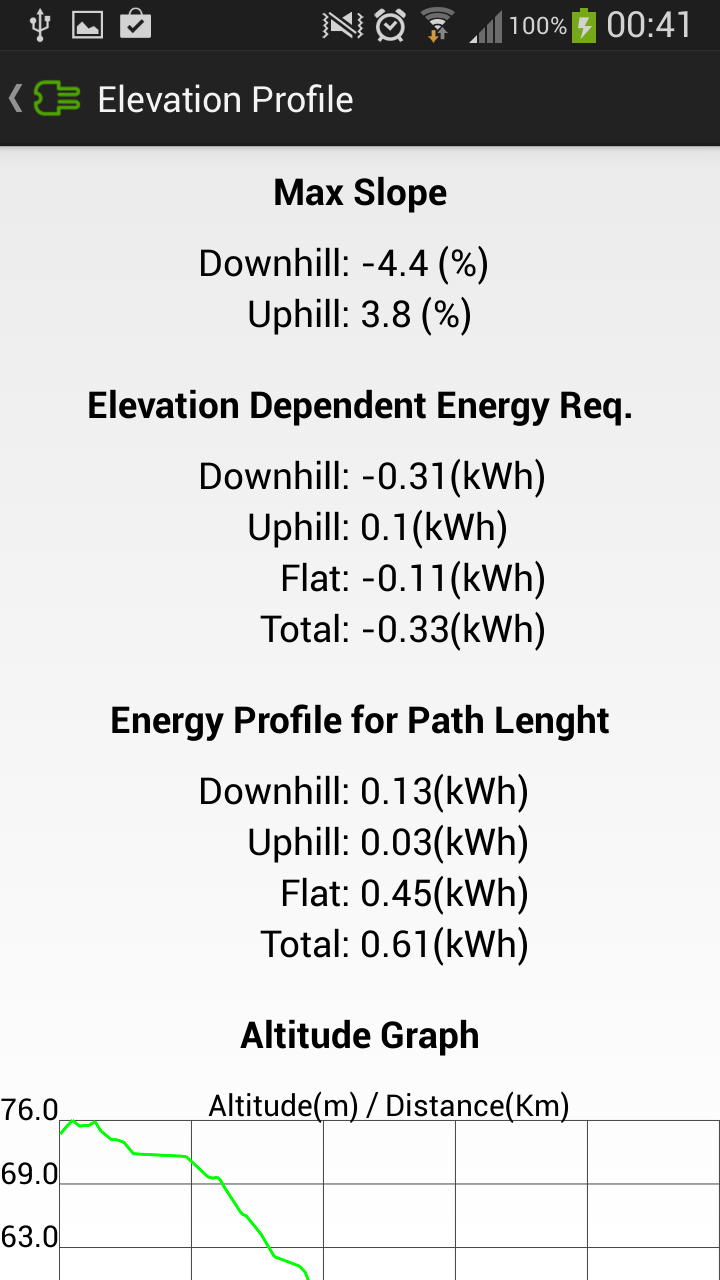
\includegraphics[width=\textwidth]{assets/mobile-app-altimetry-2.png}
		\caption{Visualizzazione opzioni di ricarica}
		\label{fig:altimetry-2}
    \end{subfigure}
	\begin{subfigure}{0.45\textwidth}
		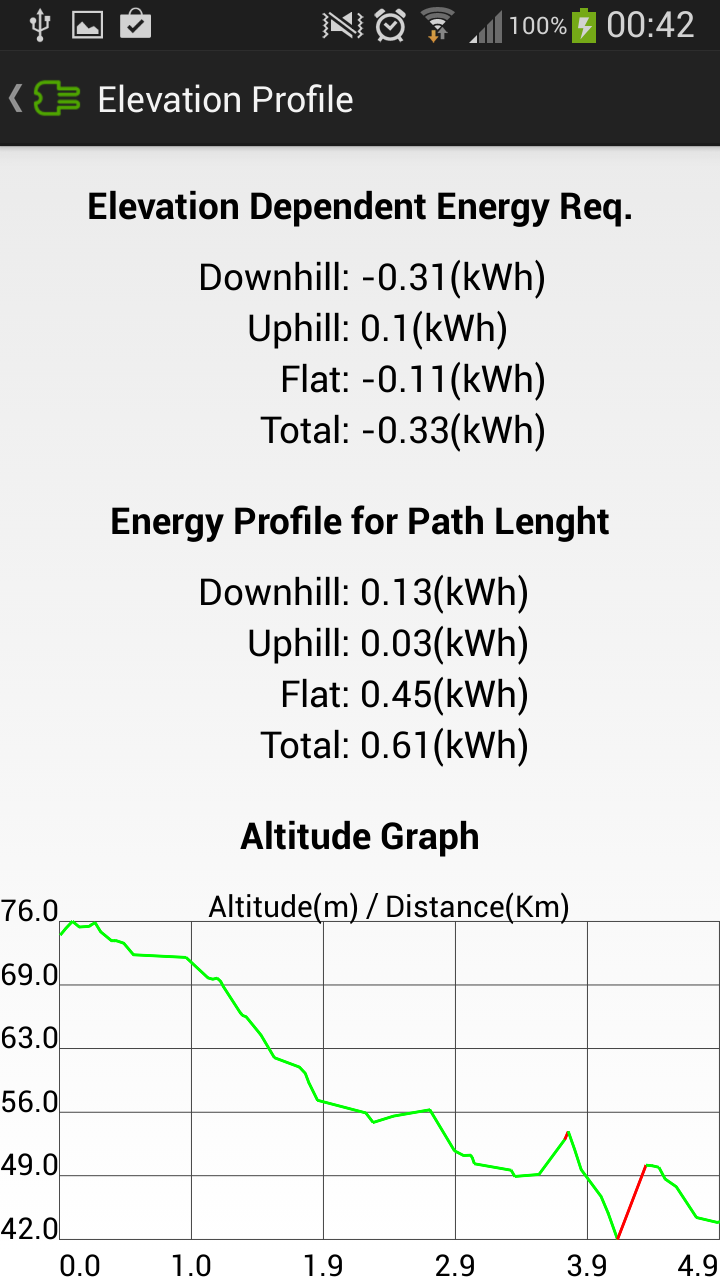
\includegraphics[width=\textwidth]{assets/mobile-app-altimetry-3.png}
		\caption{Menu opzioni di ricarica}
		\label{fig:altimetry-3}
    \end{subfigure}
\end{figure}

\subsection{Mappa}\label{subsec:map}

La mappa, quando mostrata, viene centrata sulla città di riferimento. Su di essa si può vedere il veicolo che si muove, sia che esso sia simulato sia che sia reale. Premendo il pulsante di localizzazione in alto a destra viene effettuato lo zoom sul veicolo. La mappa può essere mostrata in diverse occasioni:

\begin{itemize}
	\item \textbf{Menu principale}: Dal menu principale si seleziona \emph{Map} e si può accedere alla mappa la quale mostrerà tutti i GCP della città e da qui potremo effettuare una prenotazione cliccando direttamente sul GCP interessato (Fig. \ref{fig:map-gcp}).
	\item \textbf{Scelta delle Opzioni Ricarica}: Quando il \emph{City Service} ci restituisce le opzioni di carica disponibili possiamo visualizzarle sulla mappa. Se scegliamo di visualizzare la mappa a partire da un opzione di ricarica allora verrà anche disegnato il percorso che ci separa dalla colonnina, altrimenti verranno visualizzate tutte le colonnine e per visualizzare il percorso dovremmo selezionare quella interessata (Fig. \ref{fig:map-altimetry}). 
	\item \textbf{Prenotazioni}: Dalla schermata delle prenotazioni pendenti possiamo visualizzare sulla mappa e volendo effettuare l'operazione di ritiro semplicemente selezionando la colonnina associata.
\end{itemize}

Come mostrato in Fig. \ref{fig:map-altimetry} viene disegnato il percorso che ci separa dalla destinazione evidenziando i tratti in discesa, rosso, in salita, verde e pianura grigio.

Premendo su una delle colonnine visualizzate nella mappe viene aperto un popup che mostra informazioni sommarie e una freccia che permette di accedere a un menu con altre opzioni (Fig. \ref{fig:map-menu}). Da questo menu si può eseguire una prenotazione, vedere i dettagli sul profilo altimetrico oppure aprire il navigatore messo a disposizione dal Sistema Operativo con partenza il punto dove ci troviamo e destinazione il punto della mappa selezionato (Fig. \ref{fig:navigator}).

\section{Notifica batteria Scarica}

Un funzionalità molto importante è quella delle notifiche che avvisano l'utente quendo la batteria sta per scaricarsi (Fig. \ref{fig:notify}). Quando la batteria scende sotto una certa soglia, che attualmente è impostata al 30\%, viene lanciata una notifica all'utente che apparirà nell'area di notifica presente nei Sistemi Operativi Android, la notifica viene lanciata nuovamente a intervalli di 5\% di batteria. Premendo sulla notifica Si apre direttamente la schermata destinata alle prenotazioni.

\begin{figure}
	\centering
	\begin{subfigure}{0.45\textwidth}
		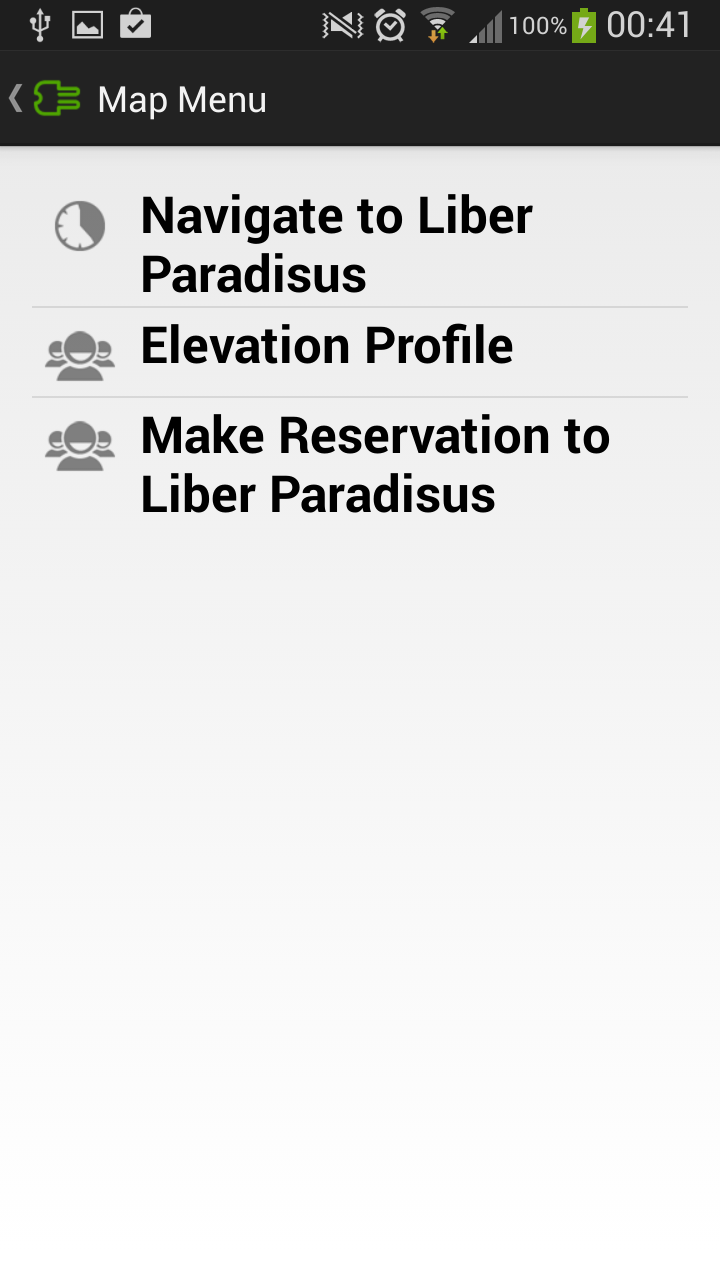
\includegraphics[width=\textwidth]{assets/mobile-app-map-menu.png}
		\caption{Menu Mappa}
		\label{fig:map-menu}
	\end{subfigure}
	\begin{subfigure}{0.45\textwidth}
		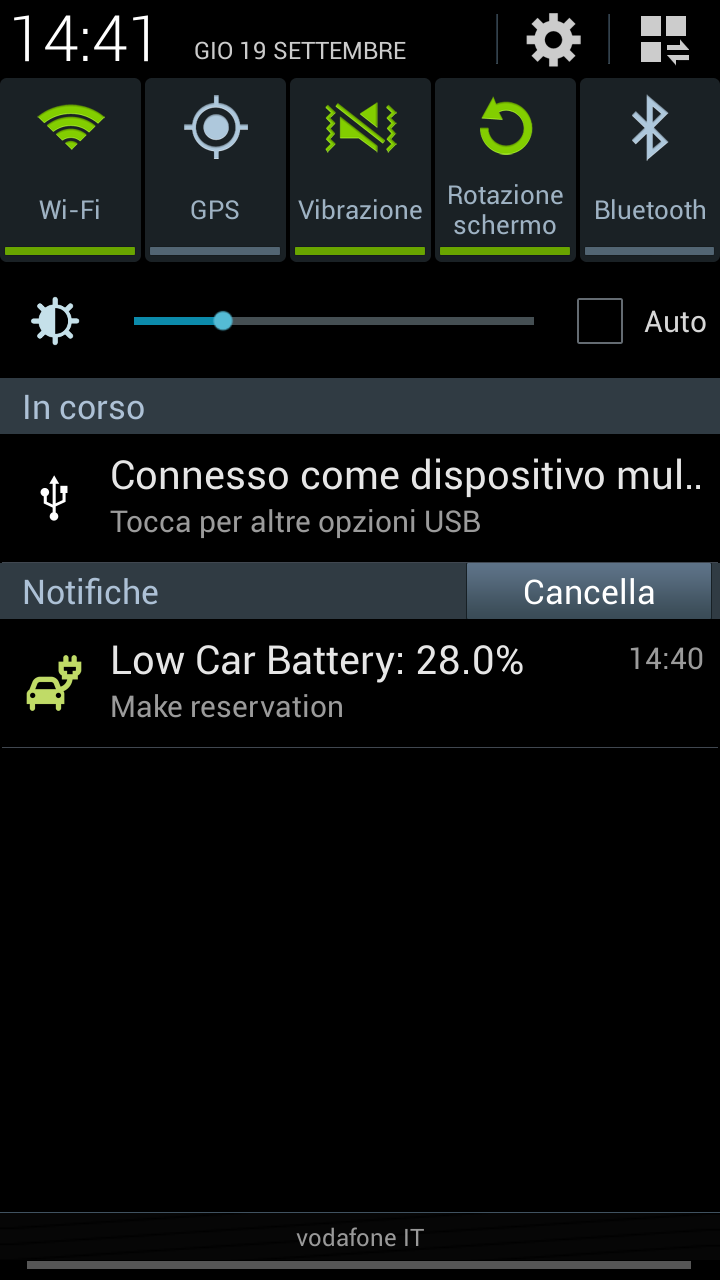
\includegraphics[width=\textwidth]{assets/mobile-app-notify.png}
		\caption{Notifica batteria scarica}
		\label{fig:notify}
	\end{subfigure}
	\begin{subfigure}{0.45\textwidth}
		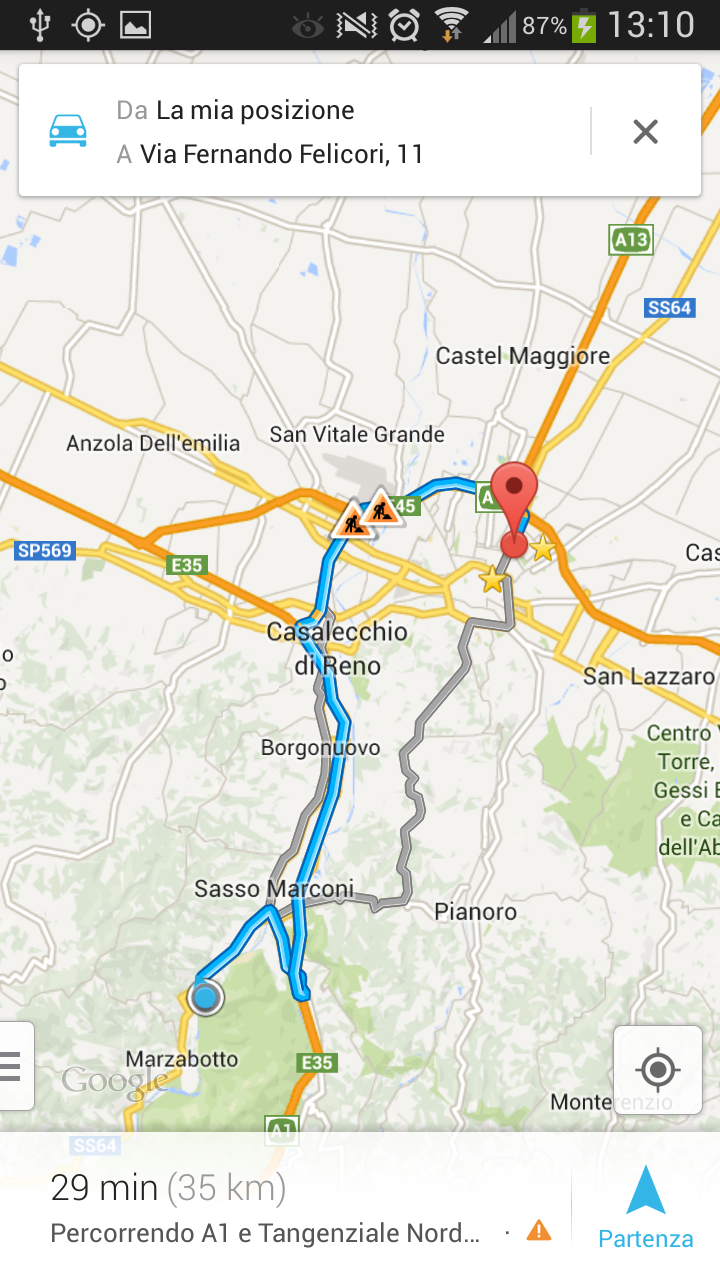
\includegraphics[width=\textwidth]{assets/mobile-app-navigator.png}
		\caption{Navigatore Satellitare}
		\label{fig:navigator}
    \end{subfigure}
	\begin{subfigure}{0.45\textwidth}
		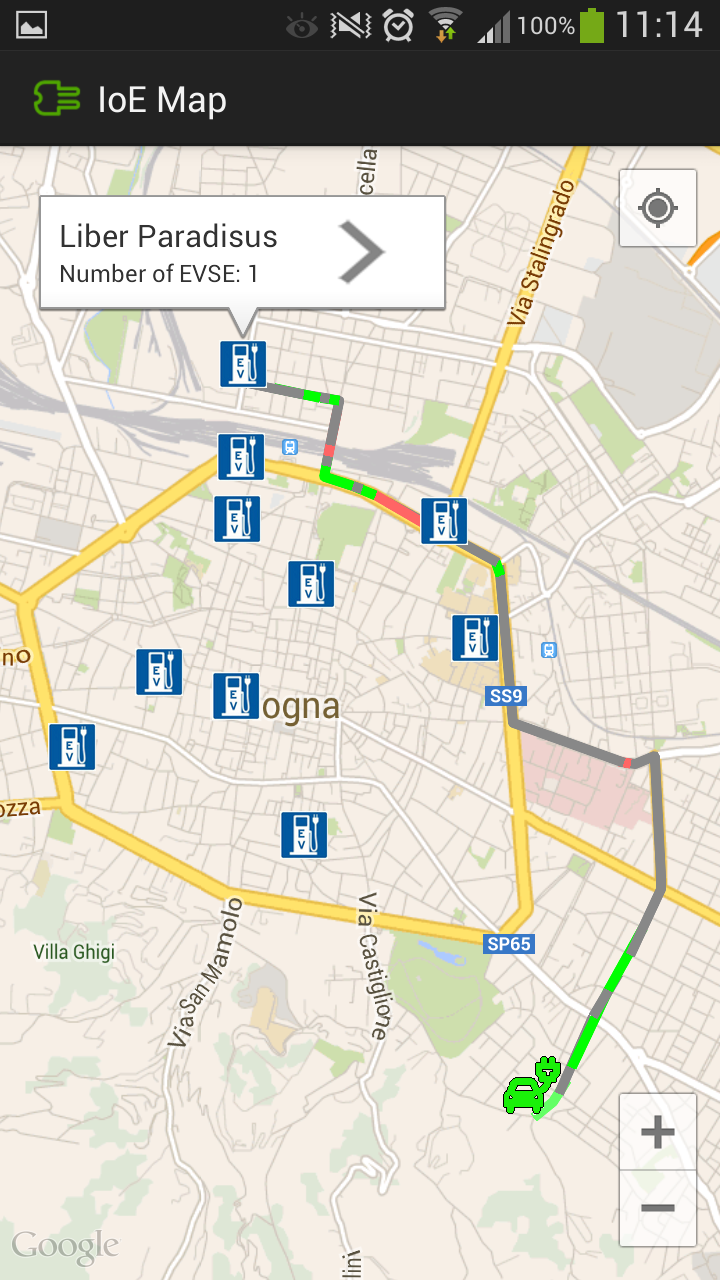
\includegraphics[width=\textwidth]{assets/mobile-app-map-gcp.png}
		\caption{Visione di tutti i GCP della città}
		\label{fig:map-gcp}
    \end{subfigure}
\end{figure}

\section{Implementazione}


\subsection{Implementazione}

\subsection{Operazioni Asincrone}

Tutte le operazioni che prevedono l'utilizzo della rete, quindi potenzialmente lunghe, sono eseguite all'interno di un \code{AsyncTask} ovvero una classe messa a disposizione dalla libreria di base di Android che permette di eseguire operazioni asincrone e contemporaneamente aggiornare l'interfaccia grafica. Questo da un lato permette di avere un applicazione fluida in quanto l'interfaccia non rimane bloccata in attesa dei risultati e dall'altro evita il verificarsi di errori dovuti al fatto che Android non permette di modificare l'interfaccia da un thread diverso da quello destinato al disegno di quest'ultima.

La maggior parte delle operazioni effettuate tramite rete, quindi nel nostro caso scambio di dati con i SIB, reperisce liste di elementi (veicoli, utenti, prenotazioni ecc..) che vengono mostrate all'interno di un apposita tipologia di Activity di Android le \code{ListActivity}.

Al fine di semplificare la programmazione delle Activity che contengono liste i quali elementi sono reperiti tramite la rete, ho creato la classe \code{ListLoaderTask<T>} che ne facilita il caricamento asincrono.

\subsection{Activities}

\subsection{Servizi}
  
  \chapter{Piattaforma di Simulazione}\label{chap:sim}

La piattaforma di simulazione è uno strumento di fondamentale importanza al fine di validare l'infrastruttura software proposta. Risulta inoltre essere un valido strumento per valutare l'impatto dell'introduzione della mobilità elettrica veicolare all'interno di un determinato contesto, grazie ad esso si può prevedere quanti veicoli sarà in grado di supportare la grid, quante colonnine saranno necessarie e che potenza dovranno avere. Risulta quindi uno strumento fondamentale sia sotto il punto di vista dell'amministrazione pubblica/cittadina, che può prevedere un piano urbanistico sostenibile, sia dal punto di vista dei gestori della rete elettrica, i quali potranno valutare la richiesta energetica di tale scenario ed eventualmente prevedere investimenti in quella direzione.

\section{Architettura}

Al fine di poter simulare gli innumerevoli aspetti legati all'Electrical Mobility sono stati usati diversi simulatori/tecnologie in simbiosi. In questa sezione verranno introdotte brevemente al fine di introdurre al resto della trattazione.

\subsection{SUMO}\label{sebsec:sumo}

SUMO (Simulator of Urban Mobility) è un simulatore Open Source e multi-piattaforma di traffico urbano progettato per simulare reti stradali di grandi dimensioni. Sviluppato in C++ è supportato principalmente dall'Institute of Transportation Systems at the German Aerospace Center. La simulazione è di tipo microscopico ovvero ogni veicolo è modellato in modo esplicito, ha un proprio itinerario e si muove individualmente attraverso la rete. Ogni aspetto relativo alla simulazione viene configurato attraverso file XML i quali descrivono la rete stradale, i parametri ed i percorsi di ogni singolo veicolo, ed eventualmente altri aspetti legati alla simulazione come i flussi di traffico oppure la descrizione degli edifici. 

SUMO permette di avviare la simulazione in due modalità:

\begin{itemize}
	\item \textbf{Visuale}: La modalità visuale permette di avere un riscontro visuale l'andamento della simulazione tramite un interfaccia che mostra la mappa della rete/città con vista dall'alto. Vengono mostrati tutti i veicoli ed è possibile accedere a tutti i parametri della simulazione. Vengono mostrati inoltre i semafori agli incroci, la segnaletica delle strade e, nel caso siano stati caricati, gli edifici della città. Tutto questo ovviamente impatta notevolmente sulle performance ma, al di la del gradevole effetto visivo, è utile per vedere come evolve la simulazione. Nel nostro caso, ad esempio, è servito per assicurarsi che i veicoli si fermassero alle colonnine, oppure per valutare la quantità di traffico generata in seguito all'inserimento di un determinato numero di veicoli. Molto utile è stato anche in fase di Demo per mostrare il funzionamento del nostro simulatore.
	\item \textbf{Testuale}: Con la modalità testuale vengono stampati nel terminale i messaggi di Warning ed Error nel terminale e se richiesto anche qualche messaggio di debug in più che indica gli step di avanzamento della simulazione. Dopo aver constatato che la simulazione si comporta come ci si aspetta tramite la modalità visuale si passa allora a questa modalità che ha performance assai maggiori. È quindi particolarmente indicata per le simulazioni di lunga durata.
\end{itemize}

\subsubsection{Tools}\label{sumo-tools}

I file XML che descrivono le simulazioni possono diventare molto complessi qualora si decida di simulare scenari realistici (come Bologna). SUMO mette a disposizione innumerevoli tool automatici per la generazione dei file di configurazione.  In questa tesi prenderemo in esame solo quelli che ci sono stati utili:

\begin{itemize}
 	\item \textbf{netconvert}: Genera file con estensione .net.xml della dove viene mappata la rete stradale. La generazione avviene in modo pseudo-casuale, tramite la definizione dei nodi e degli archi che definiscono il "grafo" della rete stradale oppure, come nel nostro caso, attraverso la conversione da formati esterni(OpenStreetMap, VISUM, VISSIM, OpenDRIVE, MATsim ecc..)
 	\item \textbf{polyconvert}: Genera file con estensione .poly.xml dove sono contenute le informazioni relative agli edifici, zone di verde, fiumi laghi ecc.. Anch'esse vengono importate dai file delle mappe in altri formati.
 	 \item \textbf{duarouter}: Genera file con estensione .rou.xml che descrivono per ogni veicolo il suo percorso, compresi tutti i suoi step intermedi. La generazione dei percorsi avviene applicando un algoritmo di cammino su grafi a scelta tra Dijikstra o A*. I punti di partenza e arrivo vengono generati casualmente da uno script in python messo a disposizione tra i tool di sumo (randomTrips.py).
\end{itemize}

\subsubsection{TRaCI}

TraCI (Traffic Controller Interface) è un modulo messo a disposizione da SUMO che permette di interagire con la simulazione in tempo reale tramite un protocollo Client/Server basato su TCP/IP. All'avvio della simulazione SUMO si mette in ascolto su una porta in attesa di messaggi, qualunque linguaggio che supporti il protocollo TCP/IP può dunque modificare lo stato della simulazione oppure ricevere notifiche sul cambiamento di variabili alle quali ci si può sottoscrivere. È proprio TraCI che farà da ponte tra SUMO e l'altro simulatore usato all'interno della nostra piattaforma.

\subsection{OMNeT++}
OMNeT++ è un ambiente OpenSource di simulazione a eventi discreti. È principalmente usato per la simulazione di reti di comunicazione, ma grazie alla sua architettura modulare ed estremamente flessibile è possibile utilizzarlo negli ambiti più disparati come la simulazione di sistemi informatici complessi, architetture hardware o, come nel nostro caso, per supporto alla simulazione veicolare.

Le simulazioni vengono modellate tramite l'impiego di componenti riusabili chiamati \emph{moduli} i quali possono essere combinati tra loro come dei blocchi LEGO.

I moduli possono essere connessi tra di loro attraverso i \emph{gates} e combinati insieme per formare dei moduli composti (compound modules). La comunicazione tra moduli normalmente avviene tramite message passing e i messaggi possono contenere strutture dati arbitrarie (a parte informazioni predefinite tipo i timestamp). Questi messaggi possono viaggiare attraverso percorsi predefiniti dai gates e dalle connections oppure essere inviati direttamente alla loro destinazione, quest'ultima scelta è molto utile nel caso delle comunicazioni wireless. 

I moduli, i relativi parametri e i collegamenti fra loro, vengono definiti tramite un linguaggio di alto livello (NED) in appositi file con estensione .ned, mentre la logica viene implementata in una corrispondente classe C++.

OMNeT++ viene distribuito con un IDE basato su Eclipse grazie al quale possono essere eseguite molte operazioni in modo visuale, come ad esempio la creazione e aggregazione di moduli.

Anche OMNeT++ mette a disposizione due modalità di esecuzione della simulazione una visuale (\emph{Tkenv}) e una testuale (\emph{Cmdenv}). La modalità visuale permette di vedere i moduli con i relativi messaggi che vengono scambiati, viene usata in fase di debug o in fase di Demo. La modalità testuale, ovviamente più performante e adatta alle simulazioni batch, mostra solo i messaggi di debug della simulazione insieme allo standard output dei moduli. Per i nostri scopi abbiamo usato solo la modalità testuale.

Un grande punto di forza di OMNeT++ sono gli strumenti messi a disposizione per l'analisi dei dati generati dalle simulazioni, che permettono di applicare, in tempo reale, trasformazioni e aggregazioni tra i set di dati e, in fine, visualizzare i risultati con varie tipologie di grafici: a barre, a linee, istogrammi e molti altri.

Ci sono due tipi di dato che si possono registrare in OMNeT++ i vettori e gli scalari, ne caso dei vettori si hanno i dati sul piano cartesiano, con il tempo come ascissa e il dato come ordinata, mentre nel caso degli scalari viene registrato un solamente un dato.

\subsection{Veins}\label{subsec:veins}

Veins è un framework OpenSource per la simulazione di reti veicolari IVC (Inter-Vehicular Communication). Utilizza OMNeT++ e SUMO in simbiosi. Si appoggia su MiXiM, un framework per OMNeT++, che implementa modelli per reti wireless fisse e mobili (reti di sensori wireless, reti ad hoc, reti veicolari ecc.). La comunicazione con SUMO avviene tramite TRaCI. Ogni volta che nella simulazione in SUMO viene aggiunto un veicolo Veins crea dinamicamente un corrispondente modulo OMNeT++ che permette di controllarlo sotto ogni aspetto (percorso, colore, velocità, accelerazione, parcheggio ecc..).

Il simulatore consiste in un modulo di Veins, il quale è stato opportunamente modificato al fine di avere un ambiente che contiene solo i componenti strettamente necessari allo scopo in quanto le performance sono determinanti al fine di poter avere dei risultati in tempi utili. Infatti sono stati rimossi da Veins i moduli necessari alla comunicazione wireless (nic80211 e ARP), il modulo per la gestione degli ostacoli (obstacles) che era utilizzato per la gestione dello shadowing delle reti wireless

\subsubsection{Il funzionamento di Veins}\label{subsubsec:veins-func}

Veins è il ponte tra OMNeT++ e SUMO e la comunicazione tra i due avviene tramite TraCI. In realtà "in mezzo" ai due simulatori si trova uno script python, \emph{sumo-launchd.py}, che sta in ascolto sulla prima porta libera che trova, in attesa che venga avviato Veins. Quando Veins viene avviato si connette a questo script il quale lancia SUMO, a questo punto inizia la sincronizzazione tra i due simulatori che avviene tramite "staffetta" come mostrato in Fig. ~\ref{fig:veins-state-machine}. Per garantire l'esecuzione sincrona a intervalli definiti Veins inserisce in un buffer tutti i comandi da inviare a SUMO (Fig.  ~\ref{fig:veins-sequence-diagram}). Ad ogni passo temporale, i comandi contenuti nel buffer vengono inviati. Ciò innesca l'avanzamento del corrispondente passo temporale nella simulazione del traffico stradale. Al termine dello step temporale di simulazione del traffico stradale, SUMO invia una serie di comandi con lo stato e la posizione di tutti i veicoli istanziati in risposta a Veins. Dopo l'elaborazione di tutti i comandi ricevuti Veins aggiunge i corrispettivi nodi per ogni nuovo veicolo introdotto nella simulazione e rimuove invece i nodi relativi ai veicoli che sono giunti a destinazione. A questo punto la simulazione può avanzare al prossimo step temporale.

\begin{figure}[H]
        \centering
        \begin{subfigure}[H]{0.5\textwidth}
                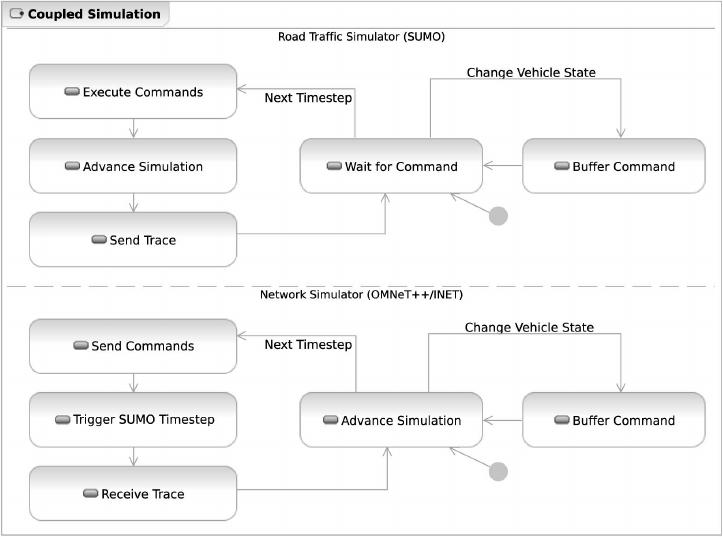
\includegraphics[width=\textwidth]{assets/veins-state-machine.jpg}
                \caption{Panoramica dei due simulatori abbinati. Macchina a stati di SUMO e i moduli di Veins.}
                \label{fig:veins-state-machine}
        \end{subfigure}%
        ~ %add desired spacing between images, e. g. ~, \quad, \qquad etc.
          %(or a blank line to force the subfigure onto a new line)
        \begin{subfigure}[H]{0.5\textwidth}
                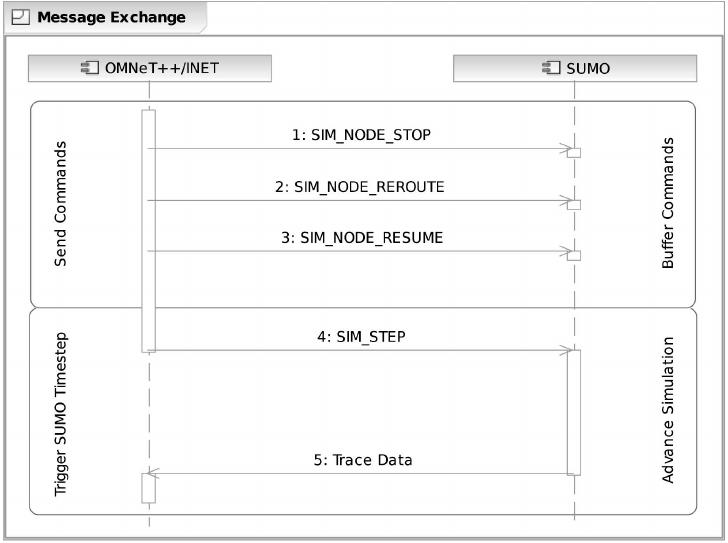
\includegraphics[width=\textwidth]{assets/veins-sequence-diagram.jpg}
                \caption{ Diagramma di sequenza dei messaggi scambiati tra SUMO e Veins. L'esecuzione dei comandi è ritardata fino al successivo passo temporale in SUMO.}
                \label{fig:veins-sequence-diagram}
        \end{subfigure}
        \caption{Architettura Veins}
\end{figure}


\section{Modellazione della Simulazione}

L'intera simulazione viene incapsulata all'interno di una Network. Il Network è lo scenario da simulare, all'interno di esso si definiscono i moduli che compongono la simulazione. Come mostrato in Fig \ref{fig:module-scenario} sono sostanzialmente 4 i moduli che compongono la nostra simulazione:

\begin{itemize}
	\item \textbf{world}: È un modulo di tipo \code{BaseWorldUtility}, fornito da MiXiM, che rappresenta l'area che circoscrive lo scenario simulato. Come configurazione richiede di definire la grandezza dello scenario in metri. La mappa usata in SUMO non può essere più grande delle dimensioni definite in questo modulo.
	\item \textbf{manager}: È un modulo di tipo \code{TraCIScenarioManagerLaunchd}, fornito da Veins, che mette in comunicazione OMNeT++ con SUMO. Tutte i messaggi inviati a TraCI passano da questo modulo (l'implementazione vera e propria della comunicazione con TraCI avviene nel modulo padre \code{TraCIScenarioManager}). Questo modulo è fondamentale in quanto è quello che crea un modulo OMNeT++ per ogni veicolo di SUMO.
	\item \textbf{cityService}: Rappresenta la grid, infatti contiene i GCP e gli EVSE. Ricopre anche la funzione di raccoglitore statistiche globali sulle colonnine e i veicoli (Sez: \ref{sec:module-city}).
	\item \textbf{connectionManager}: Questo modulo si occupa della comunicazione tra moduli ma è inutilizzato. Non l'ho rimosso per questioni di compatibilità con Veins.
\end{itemize}

Ogni volta che SUMO crea un veicolo Veins si occupa di creare il corrispondente modulo in OMNeT++, il modulo in questione è Car (Fig. \ref{fig:module-car}). Car in realtà è un modulo composto ovvero un contenitore, privo di implementazione, che contiene altri moduli. Di default, conterrebbe tutti i componenti relativi alle comunicazioni wireless in quanto sarebbe il target di Veins, ma io li ho rimossi in quanto non utili, per ora, nel nostro scenario.

Al fine di rendere la simulazione il più possibile attinente alla realtà risulta necessario implementare i modelli di carica e scarica dei veicoli e i modelli comportamentali degli utenti nonché l'implementazione dei moduli di comunicazione con il servizio cittadino. Per svolgere questi compiti è stato necessario arricchire la definizione di Car con 3 nuovi moduli:

\begin{itemize}
	\item \textbf{TraciMobility}: È un modulo fornito da Veins che mette in comunicazione il veicolo con OMNeT++ tramite TRacI.
	\item \textbf{CarLogic}: È il modulo principale, in esso è implementata la logica del veicolo. 
	\item \textbf{Battery}: Implementa il modello di carica e scarica del veicolo.
	\item \textbf{DriverBehaviour}: In questo modulo sono implementati i comportamenti che l'utente assume dinanzi a determinate scelte.  
\end{itemize}

Ogni modulo contiene dei parametri che permettono di cambiarne il comportamento, grazie a OMNeT++ diventa semplice lanciare molteplici simulazioni con diversi set di dati. Particolarmente interessante è la possibilità di eseguire la simulazione senza prenotazione per poter confrontare le differenze di occupazione delle colonnine rispetto allo scenario con prenotazione.

\begin{figure}[H]
        \centering
		\begin{subfigure}[H]{0.45\textwidth}
                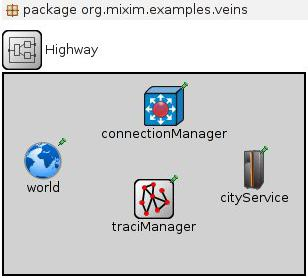
\includegraphics[width=\textwidth]{assets/module-scenario.jpg}
                \caption{Modulo scenario}
                \label{fig:module-car}
        \end{subfigure}
        \qquad
        \begin{subfigure}[H]{0.45\textwidth}
                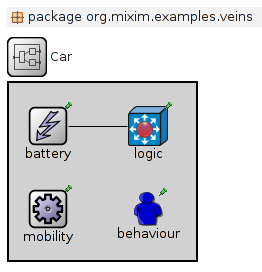
\includegraphics[width=\textwidth]{assets/module-car.png}
                \caption{Modulo Car}
                \label{fig:module-scenario}
        \end{subfigure}%
        \caption{Moduli OMNeT++}
\end{figure}

\subsection{Ciclo di Vita dei moduli}

Essendo OMNeT++ un simulatore a eventi discreti i moduli, in esso implementati, non fanno nulla finché non viene schedulato un evento. Gli eventi vengono schedulati attraverso messaggi inviati dai moduli stessi. Sostanzialmente si tratta di decidere quando, a chi e cosa mandare.
Il quando è il tempo di simulazione e quindi deve essere nel futuro o al massimo nel momento attuale di simulazione, a chi è il modulo destinatario e cosa è il messaggio da mandare. OMNeT++ fornisce un un messaggio di base, \code{cSimpleMessage}, ma, come vedremo più avanti, è possibile definirsi messaggi propri più complessi.

All'interno di questa simulazione non avviene molto scambio di messaggi tra i diversi moduli, ragion per cui risulta necessario auto-inviarsi i messaggi al fine di mantenere "vivo" il modulo.

Quando Veins crea un modulo il corrispondente veicolo in SUMO viene aggiornato ogni 0.1 secondi, che è lo step temporale di default. In OMNeT++ invece siamo noi a decidere ogni quanto aggiornare un modulo attraverso il meccanismo degli auto-messaggi. Schedulando i messaggi in modo intelligente si può guadagnare in performance in quanto ci si può inviare il messaggio solo quando è realmente necessario.

Quando un modulo Car viene creato viene chiamata la funzione \code{initialize()}, della quale il programmatore può eseguire l'override, nella quale dopo le opportune inizializzazioni, è necessario auto-schedularsi un messaggio. I messaggi vengono ricevuti dalla funzione \code{handleMessage()} alla quale viene passato un riferimento al messaggio stesso. Da dentro questa funzione si può implementare la logica del modulo. Il modulo continua a vivere finché, il corrispondente veicolo in SUMO, non giunge a destinazione momento in cui Veins, attraverso la classe \code{TraCIScenarioManager}, si accorge che il veicolo non è più nella simulazione e quindi lo elimina anche da OMNeT++ il che causa una chiamata alla funzione di terminazione \code{finish()}.

\subsection{CityService}\label{sec:module-city}

Il modulo CityService simula la grid, al suo avvio carica le informazioni relative ai GCP presenti nello scenario simulato da un file XML. Il file utilizzato è lo stesso del servizio cittadino (Sez. ~\ref{subsubsec:city-init}). Le colonnine caricate vengono trasformate in oggetti C++ al fine di poter essere usate dai veicoli virtuali. 

Questo modulo, attraverso il settaggio di parametri esterni, provvede ad abilitare/disabilitare le prenotazioni, e inoltre decide il tasso di penetrazione di veicoli elettrici nello scenario.

Quelli mostrati di seguito sono i parametri del modulo:

\begin{itemize}
	\item \code{gcpList}: Percorso del file XML che contiene la definizione dei GCP. Deve essere lo stesso utilizzato dal servizio cittadino reale.
	\item \code{electricalVehicleFreq}: Questo parametro stabilisce la frequenza con cui viene immesso un veicolo elettrico nella simulazione. È un numero che può variare da 0 a 100 e, più precisamente, indica con quale probabilità il veicolo inserito nella simulazione è elettrico. È necessario ricordare che il numero e la frequenza con cui i veicoli vengono immessi nella simulazione è determinato da SUMO attraverso i suoi file di configurazione. 
	\item \code{maxElectricalVeh}: Impone un limite superiore al numero di veicoli che possono essere presenti nella simulazione in un determinato istante. Questo significa che se è stato raggiunto il massimo numero di veicoli, e uno di questi lascia la simulazione per un qualunque motivo, allora verrà rimpiazzato da uno nuovo (sempre ammesso che SUMO generi altri veicoli e che la statistica sia favorevole). Se viene impostato a -1 allora non ci sarà nessun limite al numero di veicoli.
	\item \code{reservationEnabled}: Abilita/Disabilita il protocollo di prenotazione per i veicoli. l fine di ottimizzare le performance lo scambio di dati con il SIB, necessario per le prenotazioni, viene completamente disabilitato quando quest'ultime non sono attive.
\end{itemize}

Altra importante funzione svolta da questo modulo è la raccolta di statistiche globali sui veicoli elettrici. I dati raccolti sono tutti in formato vettoriale:

\begin{itemize}
	\item \textbf{chargingVehicles}: In questo vettore viene salvato lo stato di occupazione degli EVSE della città, ogni volta che un veicolo si va a ricaricare aggiunge un unità al vettore e quando finisce la ricarica l'unità viene rimossa. Questo comporta che come ordinata avremo al massimo il numero totale di EVSE presenti nello scenario.
	\item \textbf{electricalVehicles}: Numero di veicoli elettrici presenti nella simulazione, semplicemente ogni volta che viene aggiunto un veicolo elettrico alla simulazione viene incrementata di un unità il vettore.
	\item \textbf{vaporizedVehicles}: I veicoli vaporizzati sono quei veicoli che hanno terminato la batteria e quindi vengono letteralmente vaporizzati. Il termine vaporizzati deriva dall'analogo comando di TRacI che permette di rimuovere un veicolo dalla simulazione. 
	\item \textbf{leavingVehicles}: Questo veicolo tiene traccia dei veicoli che riescono a lasciare normalmente la simulazione ovvero arrivano a destinazione, evento che ne causa la rimozione da parte di SUMO. In realtà uno degli obbiettivi raggiunti è stato proprio quello di dirottare i veicoli che arrivano a destinazione verso una strada casuale. Non è sempre possibile intercettare l'arrivo del veicolo in una determinata strada, questo comporta che qualcuno di essi "sfugga" e venga rimosso dalla simulazione.
\end{itemize}


\subsection{CarLogic}

Il comportamento del veicolo è definito dal modulo CarLogic. Questo modulo implementa tutta la logica relativa alla guida del veicolo. In esso sono contenute le informazioni che ne descrivono la tipologia, l'appartenenza, e alcuni comportamenti di base. I comportamenti più complessi sono delegati al modulo DriverBehviour.

\begin{itemize}
	\item \textbf{userName}: Nome dell'utente che possiede il veicolo
	\item \textbf{userId}: Identificativo dell'utente che possiede il veicolo
	\item \textbf{manufacturer}: Casa produttrice del veicolo
	\item \textbf{model}: Modello del veicolo
	\item \textbf{cRoll}: Resistenza attrito gomme su asfalto
	\item \textbf{cDrag}: 
	\item \textbf{across}: Sezione frontale del veicolo
	\item \textbf{rhoAir}: Resistenza dell'aria
	\item \textbf{weight}: Peso del veicolo
	\item \textbf{threshold}: Soglia sotto la quale il veicolo si considera scarico e quindi diviene necessario fare una ricarica. Varia da 0 a 1.
	\item \textbf{minRequestedEnergyKwh}: Quantità minima di energia richiedibile in una richiesta di prenotazione. Questo valore serve nei casi in cui una richiesta non venga accettata dal \emph{City Service}, in tal caso viene diminuita gradualmente la quantità di energia richiesta fino ad arrivare a questa soglia.
	\item \textbf{writeCarStatusOnSib}: Dice se scrivere le informazioni di stato dei veicoli sul \emph{Dash SIB}. Questo permette di vedere lo stato dei veicoli dall'applicazione mobile. Essendo la scrittura sul SIB un operazione abbastanza onerosa è meglio tenere disattivata questa opzione a meno che non si sia in fase di demo.
\end{itemize}


\subsubsection{Inizializzazione}

In fase di inizializzazione la prima cosa che viene fatta è prendere un riferimento a tutti i moduli necessari, tra i quali il CityService, che  deciderà se il veicolo sarà elettrico o meno. Nel caso in cui sia elettrico allora si procede a reperire tutti i parametri e se è abilitata la prenotazione vengono scritte le informazioni del veicolo sul \emph{Dash SIB}. Viene inoltre mandato un comando a SUMO colora il veicolo di verde, funzionalità molto utile sia in fase di debug che in fase di demo.

Nel caso in cui il veicolo non sia elettrico allora vengono eliminati i relativi moduli da OMNeT++ ma il veicolo rimane in SUMO. Questa funzionalità non era prevista da Veins e quindi è stato necessario modificarlo opportunamente per introdurla. L'eliminazione avviene indirettamente, dal momento che un modulo di Veins non può eliminare se stesso, mandando un messaggio al CityService con la richiesta di eliminazione.

Un problema di SUMO, almeno per quelli che sono i nostri obbiettivi, è che un veicolo una volta giunto alla sua destinazione viene eliminato dalla simulazione. Questo comportamento influisce negativamente sulla simulazione in quanto a noi interessa simulare un periodo di vita dei veicoli lungo abbastanza da poterne studiare diversi cicli di carica e scarica. Per sopperire a questo problema vengono ottenuti, tramite TraCI, gli ID di tutte le strade che compongono il percorso del veicolo e viene preso l'ultimo in modo da poter intercettare l'arrivo del a quest'ultimo e quindi dirottarlo verso un'altra destinazione casuale. Le altre destinazioni vengono scelte da una lista che viene riempita con gli ID elle strade di destinazione, prese dai veicoli stessi, più lunghe di 50 metri. Il controllo sulla lunghezza serve in quanto è più probabile intercettare il momento in cui il veicolo arriva  a destinazione.

A questo punto come ultima operazione viene istanziato un messaggio di tipo \code{CarMessage}, appositamente creato per mantenere lo stato del veicolo attraverso le varie transazioni di stato. I campi del messaggio vengono inizializzati e il messaggio viene schedulato al tempo attuale di simulazione. Come si vede nel List. \ref{lst:omnet-msg} il messaggio viene creato, viene impostato lo stato del veicolo (Sez. \ref{subsubsec:veh-state}), e infine viene schedulato tramite la funzione \code{scheduleAt()} al tempo attuale di simulazione che viene fornito dalla funzione \code{simTime()}. Per schedulare il messaggio dopo 25 secondi sarebbe stato necessario usare \code{simTime() + 25}.

\begin{cpp}[caption={Autoschedulazione Messaggio},label={lst:omnet-msg}]
carMessage = new CarMessage("CarMessage");
carMessage->setCarState(CarState::DRIVING);
[...]
scheduleAt(simTime(), carMessage);
\end{cpp}


\subsubsection{Gli stati del veicolo}\label{subsubsec:veh-state}

Lo stato del veicolo è definito da un automa a stati finiti come mostrato in Fig. \ref{fig:car-fsmd}. Le transazioni tra gli stati avvengono tramite scambio di messaggi nei quali è definito lo stato successivo. I messaggi arrivano alla funzione \code{handleMessage} la quale controlla se il messaggio arriva dall'esterno oppure se è auto-inviato (\code{msg->isSelfMessage()}). In quest'ultimo caso allora il messaggio viene inoltrato a una funzione chiamata \code{handleSelfMessage()}. All'interno di quest'ultima funzione avviene la scelta di quale hanlder eseguire in base allo stato definito nel messaggio (Lst. lst:self-msg).

\begin{cpp}[caption={Funzione di scelta dello stato}, label={lst:self-msg}]
void CarLogic::handleSelfMessage(cMessage *msg) {
	CarMessage* carMsg = check_and_cast<CarMessage *>(msg);
	
	switch (carMsg->getCarState()) {
		case CarState::DRIVING:
			handleDriving(carMsg);
			break;
		[...]
		case CarState::CHARGING:
			handleCharging(carMsg);
			break;
		default:
			error("Unknown Car State!");
			break;
	}	
}
\end{cpp}

Ogni stato del veicolo ha una sua funzione "handler" che ne determina il comportamento. Alla funzione viene passato un riferimento al messaggio che contiene informazioni sullo stato del veicolo. L'handler prima di finire rischedula il messaggio con un nuovo stato, o con lo stesso in alcuni casi. La Fig. \ref{fig:car-fsmd} mostra l'automa a stati finiti che descrive il veicolo. 

\begin{itemize}
	\item
\end{itemize}

\begin{figure}
	\centering
	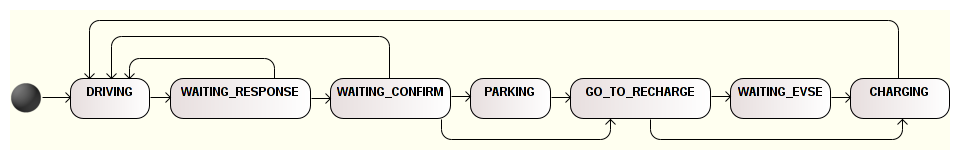
\includegraphics[width=1.0\textwidth]{assets/car-fsmd.png}
	\caption{Automa a stati finiti che descrive il veicolo, tutti gli stati possono essere finali.}
	\label{fig:car-fsmd}
\end{figure}

\subsection{Battery}\label{sec:battery}

\subsection{DriverBeahviour}

\section{Implementazione}

????
Esisteva già una versione del simulatore ma era a puro titolo dimostrativo e di demo e soffriva del fatto che era stato sviluppato da diverse persone (me compreso) in tempi molto brevi e con deadline che corrispondendo a demo internazionali si era costretti a rispettare. Questo ha portato ad avere un codice farraginoso e pieno di memory leak. Basti pensare che la prima versione del simulatore allocava RAM esponenzialmente e già dopo 2000 secondi si poteva arrivare ad avere un occupazione di 4GB.

La prima cosa che ho fatto, quando ho capito che la situazione stava diventando ingestibile è stato profilare e rifattorizzare il codice. La profilazione è avvenuta tramite il tool Valgrind grazie al quale sono riuscito ad ottenere un cosumo di memoria lineare, infatti, dove prima venivano occupati 4GB, sono riuscito a raggiungere il traguardo dei 100MB. La rifattorizzazione del codice invece è stata più complessa in quanto diverse mani hanno messo mano con diversi stili di programmazione. 

\subsection{Logging}

\subsection{SibController}

\subsection{GcpController}

\subsubsection{GCP e EVSE}

\subsection{Utility}

\section{L'ambiente di simulazione}

In questa sezione verranno descritti in dettaglio i componenti necessari a creare un ambiente di simulazione funzionante.

La logica del simulatore è implementata attraverso moduli di OMNeT++. Grazie ad essi sono implementati, i modelli di consumo dei veicoli elettrici, i comportamenti degli degli autisti e la rete di distribuzione elettrica cittadina. L'unico aspetto non implementato è la guida dei veicoli in quanto è gestita da SUMO.

I file di configurazione di SUMO sono generati da script che in base ai parametri specificati possono variare l'intensità del traffico.


\subsection{Generazione file di Configurazione}

Dopo aver scaricato compilato ed installato tutti i componenti è necessario generare i file di configurazione riguardanti lo scenario che si vuole simulare. 

\subsection{Download Scenario}

A questo punto è necessario scegliere quale scenario si vuole simulare. Lo scenario di Bologna è già disponibile nella cartella \code{simulator/veins-2.1/examples/veins/bologna} siccome è quello di nostro interesse.

Nel caso in cui si sia interessati ad uno scenario diverso da quello di Bologna il modo più semplice per ottenere la mappa desiderata è andare all'indirizzo \url{http://www.openstreetmap.org/export} e scaricarsi l'area interessata. La dimensione delle mappe scaricabili è limitata onde evitare la saturazione della banda del server. Per sopperire a questa mancanza SUMO mette a disposizione un tool situato in \code{<SUMO_HOME>/tools/import/osm/osmGet.py} che permette di scaricare mappe di dimensione arbitraria. Per l'utilizzo di questo tool rimando alla documentazione dello script oppure alla pagine ufficiale:

\url{http://sumo-sim.org/userdoc/Networks/Import/OpenStreetMapDownload.html}.

\subsubsection{Profilo Altimetrico}\label{profilo-altimetrico}

Da notare che le mappe di Open Street Map non contengono le informazioni relative al profilo altimetrico. È quindi necessario "arricchire" la mappa scaricata con tali informazioni. Il programma utilizzato a questo scopo è Osmosis, presente nella cartella \code{osmosis} del progetto. In particolare ho usato \code{osmosis-srtm-plugin_1.1.0} che permette, attraverso l'interrogazione di file SRTM (scaricabili da \url{http://dds.cr.usgs.gov/srtm/version2_1/SRTM3/}, di inserire i dati del profilo altimetrico nelle mappe di Open Street Map. 

Di seguito viene mostrato l'utilizzo del Osmosis e del relativo plugin considerando \code{\$SRTM_HOME} la cartelle che contiene i file SRTM e \code{\$CITY_NAME} il nome della città. Quindi avendo, ad esempio, \code{bologna.osm}, ovvero la mappa della città di Bologna senza dati riguardanti il profilo altimetrico, in output avremo \code{bologna_srtm.osm}, ovvero la stessa mappa con i dati estratti dai file SRTM.

\begin{bash}
osmosis -plugin org.srtmplugin.osm.osmosis.SrtmPlugin_loader --read-xml "\$CITY_NAME".osm --write-srtm locDir="\$SRTM_HOME" locOnly=true repExisting=false --write-xml "\$CITY_NAME"_srtm.osm
\end{bash}

%

Da tenere in considerazione il fatto che il comando mostrato è incluso nello script di generazione automatica da me creato al fine di velocizzare la configurazione dello scenario.

\subsection{Generazione XML di SUMO}

SUMO necessita di file di configurazione in XML che descrivono la rete stradale, i poligoni dei palazzi e i percorsi di ogni singolo veicolo. Siccome ognuno di questi file, per essere generato, richiede un apposito comando il quale a sua volta richiede vari parametri, ho creato uno script che data la mappa di una città in formato Open Street Map esegue tutte le operazioni necessarie.

Verranno comunque analizzati tutti i comandi singolarmente in modo d aavere una panoramica sulle scelte implementative.

\subsubsection{La rete Stradale (.net.xml)}

Il file della rete stradale viene generato attraverso il tool \code{netconvert} direttamente dalla mappa di Open Stree Map. Oltre al file \code{.osm} è necessario anche un file di supporto che istruisca SUMO sui vincoli e i limiti di velocità delle strade importate. Noi ne utilizziamo uno creato ad hoc per il traffico tedesco. 

Qui sotto ne riporto un frammento a puro titolo esemplificativo, il file intero si trova in \code{simulator/veins-2.1/examples/veins/bologna/osm-urban-de.typ.xml}

\begin{xml}
<types xmlns:xsi="http://www.w3.org/2001/XMLSchema-instance">
  <type id="highway.motorway" priority="13" numLanes="2" speed="41.667"
                oneway="true" disallow="bicycle pedestrian"/>
  <type id="highway.motorway_link" priority="8" numLanes="1" speed="13.889"/>
  <type id="highway.trunk" priority="12" numLanes="2" speed="13.889"/>
  <type id="highway.trunk_link" priority="8" numLanes="1" speed="13.889"/>
  <type id="highway.primary" priority="11" numLanes="2" speed="13.889"/>
  <type id="highway.primary_link" priority="8" numLanes="1" speed="13.889"/>
  <type id="highway.secondary" priority="10" numLanes="2" speed="13.889"/>
  ....
</types> 
\end{xml}

Di seguito passiamo ad un analisi dettagliata di tutti i parametri passati a \code{netconvert}:

\begin{itemize}
	\item \textbf{-{}-type-files}: Specifica il file che contiene i vincoli e i limiti, quello citato sopra.
	\item \textbf{-{}-ramps.guess}: Prova a capire dove sono le rampe e ad eseguirne l'importazione
	\item \textbf{-{}-remove-edges.by-vclass}: Siccome Open Street Map include un infinità informazioni del tutto inutili al nostro fine (ferrovie, piste ciclabili, aree pedonali ecc..) con questo parametro si indicano le classi da non importare (\code{bicycle,pedestrian...})
	\item \textbf{-{}-geometry.remove}:
	\item \textbf{-{}-remove-edges.isolated}:
	\item \textbf{-{}-tls.join}:
	\item \textbf{-{}-osm-files}:
	\item \textbf{-{}-output.street-names}:
	\item \textbf{-{}-output.original-names}:
	\item \textbf{-{}-output-file}:
\end{itemize}

Siccome Open Street Map include molte informazioni che sono del tutto inutili al nostro fine (ferrovie, piste ciclabili, aree pedonali ecc..) bisogna istruire \code{netconvert} affinché le escluda dall'importazione. 

%\begin{bash}
%netconvert --type-files osm-urban-de.typ.xml --ramps.guess --remove-edges.by-vclass hov,taxi,bus,delivery,transport,lightrail,cityrail,rail_slow, rail_fast,motorcycle,bicycle,pedestrian --geometry.remove --remove-edges.isolated true --tls.join --osm-files "$MAP_FILE" --output.street-names --output.original-names --output-file "$CITY_NAME".net.xml
%\end{bash}


  
  \appendix%tutti i capitoli da qui in avanti sono considerati appendici
  
  \chapter{Installazione Ambiente}

\section{Installazione}

Per far interagire tutti gli elementi necessari alla simulazione è necessario installare numerosi framework e librerie. In questa sezione verrà data una guida il più esaustiva possibile per installare e configurare un ambiente funzionante. Verranno inoltre forniti i link specifici per l'installazione di ogni componente qualora insorgano delle problematiche.

Il procedimento di installazione è testato e funzionante su Debian \emph{7} Wheezy (con versioni precedenti potrebbero esserci problemi con le versioni delle librerie) e Ubuntu dalla versione \emph{12.10} alla \emph{13.10}. È stato anche possibile completare l'installazione su MacOSX ma non essendomene occupato personalmente non posso assicurare nulla al riguardo.

\subsection{Installazioni preliminari}

Questi sono i pacchetti che vanno installati su Debian 7 al fine di installare tutti i componenti successivi. Non è sicuro che siano gli unici necessari. È probabile che lo stesso comando vada bene anche per Ubuntu.

\begin{bash}
sudo apt-get install bison flex build-essential zlib1g-dev tk8.4-dev blt-dev libxml2-dev libpcap0.8-dev autoconf automake libtool libxerces-c2-dev libproj-dev libproj0 libfox-1.6-dev libgdal1h libboost-dev
\end{bash}

\subsection{OMNeT++} 

AL momento di scrivere questo documento la versione usata per il progetto è la 4.4 ma in generale le versioni dalla 4.2 in su dovrebbero andare bene. Questo è il link per la versione 4.4 \url{http://www.omnetpp.org/omnetpp/cat_view/17-downloads/1-omnet-releases}. Dopo aver scaricato il tar.gz lo si estragga e si proceda con l'installazione:

\begin{bash}
./configure
make
bin/omnetpp
\end{bash}

\bigskip
\noindent
Durante l'installazione verrà detto di inserire alcune variabili d'ambiente nel file .bashrc non dimenticarsi di eseguire queste direttive.

In Ubuntu 13.10 si può assistere a un bug che determina la sparizione dei menu di OMNeT++, per risolverlo è necessario impostare la seguente variabile d'ambiente nel file  \code{$\sim$/.basrc}:

\begin{bash}
export UBUNTU_MENUPROXY=0
\end{bash}

\noindent
per maggiori informazioni guardare questa discussione su StackOverflow \url{http://stackoverflow.com/questions/19452390/eclipse-menus-dont-show-up-after-upgrading-to-ubuntu-13-10}

\subsection{SUMO}

Seppur SUMO sia disponibile tra i pacchetti di Debian/Ubuntu è necessario comunque scaricare i sorgenti tramite SVN di una versione successiva alla \emph{15340} e compilarli. Questo perchè la versione attualmente disponibile tramite il gestore di pacchetti, ovvero la \emph{0.19.0}, non supporta l'importazione nelle mappe (i file .net.xml) dei dati del profilo altimetrico, fondamentali per avere un modello di consumo energetico del veicolo realistico.

Quindi i comandi necessari, presupponendo di avere Subversion installato, sono:

\begin{bash}
svn co https://sumo.svn.sourceforge.net/svnroot/sumo/trunk/sumo
make -f Makefile.cvs
./configure
make
sudo make install
\end{bash}

Per una trattazione più completa dell'installazione rimando il sito ufficiale \url{http://sourceforge.net/apps/mediawiki/sumo/index.php?title=Installing/Linux_Build}

\subsection{SMART-M3}

La tecnologia Smart-M3 forisce la SIB, ovvero il database semantico usato per lo scambio di informazioni tra i vari componenti del sistema. Noi utilizzeremo nello specifico la RedSIB sviluppata da ARCES e basata su un progetto di Nokia
(Nokia C Smart M3).
La versione supportata dal nostro ambiente è la 0.9 ma anche le successive dovrebbero andare bene. Il link per il download è questo: \url{http://sourceforge.net/projects/smart-m3/files/Smart-M3-RedSIB_0.9/}. Una volta estratto il tar.gz al suo interno troveremo sia i sorgenti che i pacchetti per Debian. Nel caso si intenda compilare i sorgenti rimando alle istruzioni contenute all'interno del pacchetto. Qui ci limiteremo a installare i deb attraverso gli script forniti:

\begin{bash}
sudo ./install.sh     #per architetture x86
sudo ./install_x64.sh #per architetture amd64
\end{bash}

All'interno del pacchetto viene data la possibilità di utilizzare Virtuoso come database RDF ma, seppur probabilmente sia più performante, non lo utilizzeremo in quanto è una feature introdotta recentemente e quindi non abbastanza testata.

\subsection{KPI_Low}

La libreria KPI_Low è un API scritta in C che, attraverso il protocollo SSAP, permette di interfacciarsi alla SIB. È stata scritta da Jussi Kiljander, un ricercatore del VTT Technical Research Centre of Finland, e successivamente modificata da Federico Montori di UNIBO per aggiungervi il supporto alle query SPARQL. Io l'ho modificata al fine di rimuovere dei Memory Leak trovati grazie al tool Valgrind.
In quanto la versione della libreria non è quella originale è necessario usare la nostra versione che si trova nella cartella \code{kpi_low_mod} nella root del progetto.
Le KPI_Low necessitano della libreria SCEW per il parsing XML, la quale non si trova nei repository di Debian/Ubutnu,  è quindi necessario scaricarla dal seguente indirizzo \url{http://nongnu.askapache.com/scew/scew-1.1.3.tar.gz} e compilarla. Una volta scaricata estrarla e spostarsi nella cartella estratta:

\begin{bash}
./configure
make
sudo make install
\end{bash}

Adesso possiamo procedere con l'installazione delle KPI_Low, spostarsi dunque nella cartella \code{kpi\_low\_mod}:

\begin{bash}
./autogen.sh
./configure
make
sudo make install
\end{bash}

per istruzioni più dettagliate guardare il documento \code{kpi_low_mod/KPI_Low.pdf}

\subsection{Importare il progetto in OMNeT++}

Adesso che abbiamo predisposto l'ambiente possiamo procedere con l'importazione in OMNeT++ del simulatore e con la compilazione. Apriamo OMNeT++, se è il primo avvio ci chiederà che Workspace usare proponendocene uno predefinito, in tal caso noi scegliamo la cartella \code{simulator} all'interno della root del progetto. Probabilmente verrà chiesto anche se si vuole abilitare il supporto ai framework MiXiM e INET e se si vogliono importare i porgetti di esmpio, in entrambi i casi diciamo di no. Nel caso in cui il workspace fosse già impostato allora andiamo su \code{File -> Switch Workspace -> Other...} e selezioniamo la cartella \code{simulator} nella root del progetto proprio come sopra. Se a seguito della selezione del workspace \code{simulator} la scheda dei progetti rimane vuota allora andiamo su \code{File -> Import... -> General/Existing Project into Workspace -> Next} e come root directory scegliamo \code{simulator}, dovremmo vedere il progetto \code{veins-2.1} nel riquadro \code{Projects}, lo selezioniamo e clicchiamo su \code{Finish}.

A questo punto non rimane che compilare il progetto. La compilazione può avvenire in due modalità:

\begin{itemize}
	\item \textbf{gcc-debug}: Compila includendo le informazioni di debug rendendo possibile l'utilizzo di \code{gdb} per analizzare il funzionamento del programma. OMNeT++ mette a disposizione un front-end visuale per \code{gdb} che permette di inserire breakpoint nel sorgente ed eseguire l'avanzamento step a step. Inoltre permette di visualizzare il contenuto delle variabili durante l'esecuzione semplicemente semplicemente spostando il cursore sulla variabile interessata nel riquadro dei sorgenti. Queste funzionalità sono da prendere seriamente in considerazione qualora, a seguito di modifiche, la simulazione dovesse fallire.
	\item \textbf{gcc-release}: Compila non includendo le informazioni di debug e applicando le ottimizzazioni previste dal compilatore \code{gcc} con il flag \code{-O2}. Ovviamente questa configurazione è più performante della precedente e andrebbe usata quando, una volta ritenuto stabile il codice, si vogliono eseguire simulazioni batch.
\end{itemize}

Il cambio di modalità di compilazione si può effettuare tramite: \code{Tasto DX su veins-2.1 -> Build Configurations -> Set Active -> gcc-debug/gcc-release}.

I file che fanno parte del simulatore si trovano sotto la directory \code{simulator/veins-2.1/examples/veins}. 

\chapter{Vista al Centro Ricerche Fiat}\label{app:crf}

\chapter{UniboGeoTools}\label{app:unibo-geo-tools}

Libreria java sviluppata per motivi strani

\chapter{OntologyLoader}\label{app:ontology-loader}


\chapter*{\refname}
\printbibliography[heading=cartaceo,nottype=online]
\printbibliography[heading=web,type=online]

  
\end{document}